\documentclass{article}

% General package includes
\usepackage{amsmath}
\usepackage{amssymb}
\usepackage{amsfonts}
\usepackage{mathtools}
\usepackage{fontspec}
\usepackage{changepage}
\usepackage{todonotes}
\usepackage{mathpartir}
\usepackage{mdframed}
% needed for some symbols in Iris
\usepackage{stmaryrd}
\usepackage{array}
\usepackage{makecell}
\usepackage{cancel}
\usepackage{xcolor}
\usepackage{longtable}

% Moving figure captions closer to the contents.
\usepackage[skip=3pt]{caption}

% Styling links
\usepackage{hyperref}
\hypersetup{
    %colorlinks=true,
    linkcolor=black,
    citecolor=black,
    %filecolor=magenta,      
    urlcolor=blue,
    % frenchlinks=true
    }
\urlstyle{same}

% For bibliography
\usepackage{biblatex}
\addbibresource{thesis.bib}

% Settings page size
\usepackage{geometry}
\geometry{a4paper, margin=3cm}

% For including images
\usepackage{graphicx}
% https://www.overleaf.com/learn/latex/Inserting_Images#The_folder_path_to_images
\graphicspath{{./images/}}

% Font configuration
\usepackage[
    math-style=ISO,
    bold-style=ISO,
    partial=upright,
    nabla=upright
]{unicode-math}

\setmainfont{Libertinus Serif}
\setsansfont{Libertinus Sans}
\setmathfont{Libertinus Math}
\setmathfont{Latin Modern Math}[range=\ast]
\setmonofont{Source Code Pro}
\newfontfamily\symfont{FreeMono}
\newfontfamily\symfontextra{FreeSerif}

% Define some unicode characters missing from Source Code Pro
\usepackage{newunicodechar}
\newunicodechar{∗}{{\symfont ∗}}
\newunicodechar{⊥}{{\symfont ⊥}}
\newunicodechar{⊤}{{\symfont ⊤}}
\newunicodechar{▷}{{\symfont ▷}}
\newunicodechar{↦}{{\symfont ↦}}
\newunicodechar{∨}{{\symfont ∨}}
\newunicodechar{∈}{{\symfont ∈}}
\newunicodechar{γ}{{\symfont γ}}
\newunicodechar{Φ}{{\symfont Φ}}
\newunicodechar{⊢}{{\symfont ⊢}}

  
% For including source code blocks
\usepackage{minted}
\usepackage{xpatch}
% Remove latex indent for source code
\setminted{autogobble,linenos,fontsize=\footnotesize}
% Define inline shortcuts without syntax highlighting
\newmintinline[ocamlin]{text}{fontsize=\footnotesize}
\newmintinline[ocamlreal]{ocaml}{fontsize=\footnotesize}
\newmintinline[coqin]{text}{}
% disable comments using italics
% from https://tex.stackexchange.com/a/469702
\xpatchcmd{\minted}{\VerbatimEnvironment}{\VerbatimEnvironment\let\itshape\relax}{}{}

\BeforeBeginEnvironment{minted}{\begin{mdframed}}
\AfterEndEnvironment{minted}{\end{mdframed}}

% Iris/separation logic definitions
\usepackage{iris}

% Some custom shortcuts
\newcommand{\hazel}{Hazel}
\newcommand{\CC}{C\nolinebreak\hspace{-.05em}\raisebox{.2ex}{\small\bf +}\nolinebreak\hspace{-.10em}\raisebox{.2ex}{\small\bf +}}
\newcommand{\ocf}{OCaml~5}
\newcommand{\done}{{\symfontextra ✓}}
\newcommand{\tbd}{{\symfontextra ⌛}}
\newcommand{\efork}{\emph{Fork}}
\newcommand{\esuspend}{\emph{Suspend}}
\newcommand{\egetctx}{\emph{GetContext}}
\newcommand{\proto}{\emph{Coop}}
\newcommand{\protod}{\emph{Coop}~\ensuremath{\delta}}
\newcommand{\gsIsReg}{\emph{isRegister}}
\newcommand{\gsIsWaker}{\emph{isWaker}}
\newcommand{\gsIsCb}{\emph{isCallback}}
\NewDocumentCommand\ewp{O{} m O{} m m}%
  {\mathit{ewp}^{#1}_{#3}\spac\left(#2\right)\spac\left\langle#4\right\rangle\spac{\left\{#5\right\}}}
\newcommand{\ewpt}{\emph{ewp}}
\newcommand{\gsReady}{\emph{Ready}}
\newcommand{\gsPState}{\emph{PromiseState}}
\newcommand{\gsPInvIn}{\emph{PInvInner}}
\newcommand{\gsPInv}{\emph{PromiseInv}}
\newcommand{\invN}{\ensuremath{\mathcal{N}}}
\newcommand{\gsIsPr}{\emph{isPromise}}
\newcommand{\gsIsQueue}{\emph{isQueue}}
\newcommand{\gsIsCQS}{\emph{isCQS}}
\newcommand{\gspwait}{\emph{promiseWaiting}~\ensuremath{\gamma}}
\newcommand{\gspdone}{\emph{promiseDone}~\ensuremath{\gamma}}
\newcommand{\gssignal}{\emph{signalAllPermit}}
% A variable number of quads
% https://tex.stackexchange.com/a/330591
\newcommand{\myquad}[1][1]{\hspace*{#1em}\ignorespaces}

\title{Verifying an Effect-Based Cooperative Concurrency Scheduler in Iris}
\author{
    Adrian Dapprich \\
    Department of Computer Science\\
    Saarland University \\\\
    Advisors: Prof. Derek Dreyer \& Prof. François Pottier}
% \institute{Foundations of Programming Group, MPI-SWS, Saarland University}
\date{\today}

\begin{document}

% TODO better title page
\maketitle
\newpage

\tableofcontents
\newpage

\section{Introduction (WIP)}
\label{sec:introduction}

\begin{itemize}
  \item As a motivation for the work: program verification, \textbf{safety} and why we care about it.
  \item Iris is a new separation logic which allows proving safety for programs using mutable shared state.
  \item Many programs nowadays user user-level concurrency to handle a big number of tasks. As an example for \ocf{} there exists the Eio library which provides concurrency primitives using effect handlers.
  \item Effect handlers are a versatile concept which allow a modular treatment of effects, the implementation in form of a handler is separated from the code using the effect, and it's more lightweight than monads. Give a simple example of state.
        \begin{itemize}
          \item The biggest upside is that they are more composable than monads which often require rewriting of parts of the program into monadic style
          \item In theory effect can be tracked by the type system, although \ocf{} does not do that yet.
          \item Explain the concept of \textbf{effect safety} here.
          \item Explain how performing and handling effects is implemented using delimited continuations.
          \item Mention that continuations can only be invoked once? (not really necessary info)
        \end{itemize}
  \item We want to verify some parts of the Eio library but the standard Heaplang language for Iris does not support effect handlers.
        \begin{itemize}
          \item \hazel{} is an Iris language formalizing effect handlers using protocols.
          \item Syntax and semantics of protocols.
          \item Since \ocf{} allows both effect handlers and mutable shared state we had to add a multithreaded semantics to \hazel{}.
        \end{itemize}
  \item Inherent part of a scheduler is liveness, because it is responsible for running all fibers to completion. Unfortunately it is hard to prove liveness properties in Iris, so we just focus on safety and effect safety.
\end{itemize}

\subsection{The Eio Library (WIP)}
\label{sec:intro-eio}

\begin{itemize}
  \item Library for cooperative concurrency in \ocf{}.
  \item Implements switching between tasks using effect handlers.
  \item A fiber is a normal OCaml function which may perform effects that are handled by a scheduler.
  \item Each scheduler is only responsible for a single thread, more can be spawned.
  \item It offers abstractions to operating system resources to fibers, e.g. network, file system, timers etc.
  \item It also offers synchronization and message passing constructs like mutexes \& channels which are specialized to handle fibers, i.e. a mutex does not suspend the system-level thread, but the fiber.
\end{itemize}

\subsection{Focus and Structure of the Thesis}
\label{sec:intro-structure}

Eio aims to be the standard cooperative concurrency library for \ocf{}, so it includes many functions for structured concurrency of fibers (e.g. \ocamlin{Fiber.{first, any, both, all}}, which run two or more fibers and combine their results), support for cancelling fibers, abstractions for operating system resources, a different scheduler implementation per OS, and synchronization constructs like promises and mutexes.
But for this work we restrict ourselves to verifying the safety and effect safety of Eio's core functionalities:
\begin{enumerate}
  \item Running fibers in a "common denominator" scheduler that does not interact with any OS resources,
  \item awaiting the result of other fibers using the \textit{promise} synchronization construct,
  \item and spawning new schedulers to run fibers in another thread.
\end{enumerate}

\begin{figure}[ht]
  \centering
  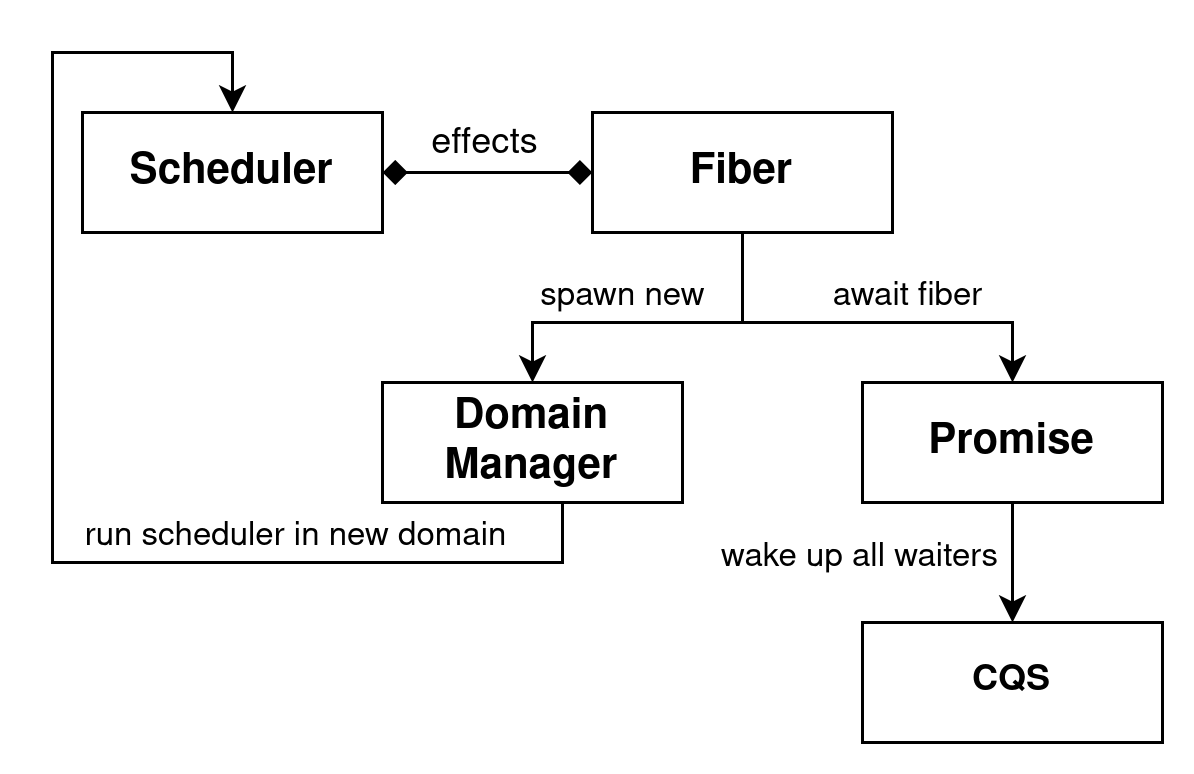
\includegraphics[width=0.75\textwidth]{Eio_Module_Hierarchy.png}
  \caption{Eio Module Hierarchy}
  \label{fig:eio-module-hierarchy}
\end{figure}

Figure~\ref{fig:eio-module-hierarchy} shows the simplified module hierarchy of the concepts we focus on.
A standard arrow stands for a direct source code dependency from one module to another.
The diamond arrow between \ocamlin{Scheduler} and \ocamlin{Fiber} stands for the implicit dependency that code in the fiber module performs effects that are handled by code in the scheduler module.

Fibers can fork off new fibers using the \efork{} effect and suspend execution using the \esuspend{} effect, which are both handled by the scheduler.
The implementation of the fiber and scheduler functions are discussed in section~\ref{sec:sched-impl}.
\textit{Promises} are built on top of the \textit{CQS} data structure, which is a lock-free condition variable that is used by fibers to suspend execution until a promise is fulfilled.
The specification of promises is discussed in section~\ref{sec:sched-spec}.
The CQS specification is already verified using Iris, but Eio uses a custom implementation for which we had to adapt the proof and we discuss this process in section~\ref{sec:cqs}.
Fibers in Eio also have access to \textit{thread-local variables} by performing a \egetctx{} effect, which is discussed in section~\ref{sec:thread-local-vars}.
They are thread-local in the sense that they are shared between all fibers of one scheduler.
Finally, we discuss our addition of multi-threading to the \hazel{} operational semantics in order to model running schedulers in different threads.
This turned out to be technically trivial, so we only discuss it in the appendix and take a multithreaded semantics and support for Iris \textit{shared invariants} as a given in the reminder of the main text.

\subsection{Contributions}
\label{sec:intro-contributions}

To summarize our contributions, in this thesis we verify the \textbf{safety} and \textbf{effect safety} of a simplified model of Eio which serves as an extended case study on the viability of \hazel{} for verifying programs with effect handlers.
This includes:

\begin{itemize}
  \item The verification of the basic Eio \textbf{fiber abstraction} running on a common denominator scheduler.
  \item An adaptation of the existing verification of CQS to the customized version used by Eio.
  \item Adding multi-threading to \hazel{}'s operational semantics, which shows we can reason about programs that use both \textbf{multi-threading} and \textbf{effect handlers}.
\end{itemize}

\section{Verifying a Basic Eio Scheduler}
\label{sec:scheduler}

Cooperative concurrency schedulers for user-level threads (i.e. \emph{fibers}) are commonly treated in the literature
on effect handlers~\cite{dolan2018concurrent,leijen2017structured,de2021separation} because they are a good example for the usefulness
of manipulating delimited continuations with effect handlers.
Generally, the scheduler contains an effect handler and fibers are normal functions which perform effects to yield execution.
Performing an effect causes execution to jump to the enclosing effect handler, providing it with the rest of the fiber's computation in the form of a delimited continuation.
The scheduler keeps track of a collection of these continuations and by invoking one of them it can schedule the next fiber.
This approach is also used in Eio.

In the following we define a basic model of the Eio scheduler and related data structures such as promises.
Throughout the thesis we then extend this model with more features.
We first discuss the implementation of our model and give an intuition about the behavior of each component in section~\ref{sec:sched-impl}.
Based on this intuition we then build a formalization in section~\ref{sec:sched-spec}.
We mechanize our development in the Coq proof assistant and use the simple cooperative concurrency scheduler case study from the dissertation of de Vilhena~\cite{de2022proof} (Chapter 4) as a basis.

\subsection{Implementation}
\label{sec:sched-impl}

Let us first get an idea of how the different core elements of Eio interact by looking at their types.
The code we present throughout the thesis is \ocf{} code that represents the \hh{} code we verify.

\begin{minted}{ocaml}
  (* Basic interface of the Eio library. *)
  Scheduler.run : (unit -> 'a) -> 'a
  Fiber.fork_promise : (unit -> 'a) -> 'a Promise.t
  Promise.await : 'a Promise.t -> 'a
\end{minted}

\ocamlin{Scheduler.run} is the main entry point to Eio.
It runs a scheduler and is provided a function which represents main fiber.
A scheduler runs the main fiber and all forked off fibers in a single thread.
However, in Eio a fiber can also spawn new schedulers in separate threads to run other fibers in parallel.
We extend our model with this feature in section~\ref{sec:domain-manager}, but in this section we already assume that fibers can run in different threads to build key data structures in a thread-safe way.

The \ocamlin{Fiber.fork_promise} function is used to spawn fibers in the current scheduler.
The function returns a promise holding the eventual return value of the new fiber.
The promise is thread-safe so that it can be shared with fibers running in different threads.
The \ocamlin{Promise.await} function can be used by any fiber to suspend execution until the value of a promise is available.
Common problems like deadlocks are not prevented in any way and are the responsibility of the programmer.

\subsubsection{\ocamlin{Scheduler.run}}
\label{sec:sched-impl-run}

\begin{figure}[ht]
  \begin{minted}[escapeinside=@@]{ocaml}
module Scheduler = struct
  type _ eff += Fork : (unit -> unit) -> unit eff
  type 'a waker : 'a -> unit
  type _ eff += Suspend : ('a waker -> unit) -> 'a eff

  let run init (main: unit -> 'a) : 'a =
    let result = ref None in
    let run_queue = Queue.create () in  @\label{ln:run_queue}@
    let rec next () =  @\label{ln:run_next}@
      match Queue.pop run_queue with
      | None -> begin
          match !result with @\label{ln:run_check}@ 
          | None -> next ()
          | Some _ -> ()
        end
      | Some fiber -> fiber () 
    in
    let rec execute fiber = @\label{ln:run_execute}@ 
      match fiber () with
      | () -> next ()  @\label{ln:run_value}@
      | @\texttt{\textbf{effect}}@ (Fork fiber), k ->  @\label{ln:run_fork}@
          Queue.push run_queue (fun () -> continue k ()); @\label{ln:run_push}@ 
          execute fiber @\label{ln:run_rec}@
      | @\texttt{\textbf{effect}}@ (Suspend register), k ->  @\label{ln:run_suspend}@
          let waker = fun v -> Queue.push run_queue (fun () -> continue k v) in @\label{ln:run_waker}@  
          register waker;  @\label{ln:run_register}@
          next ()
    in
    let tlv = ref init in
    execute (fun () -> result := Some (main ())); @\label{ln:run_main}@ 
    match !result with @\label{ln:run_return}@
    | None -> error "impossible"  @\label{ln:run_error}@
    | Some result -> result
end
  \end{minted}
  \caption{Implementation of \ocamlin{Scheduler.run}.}
  \label{fig:sched-impl-run}
\end{figure}

As mentioned above this is the main entry point to the Eio library and its code is shown in figure~\ref{fig:sched-impl-run}.
It sets up the scheduler environment and then runs the main fiber (and every subsequent fiber) under an effect handler.

The \ocamlin{result} reference eventually holds the final value of the main fiber.
The \ocamlin{run_queue} (line~\ref{ln:run_queue}) contains closures that invoke the continuation of an effect.
The closures represent ready fibers which can continue execution from the point where they performed an effect.
The \ocamlin{next} function (line~\ref{ln:run_next}) pops one fiber from the \ocamlin{run_queue} and executes it.
If no more ready fibers remain, the function will check if the main fiber has already finished execution~\ref{ln:run_check} and if so it will also exit, which causes the scheduler to return the main fiber's final value~\ref{ln:run_return}.
Otherwise, the main fiber's continuation exists \emph{somewhere} -- it could be deadlocked or just awaiting a promise from a different thread -- so the \ocamlin{next} function busy loops until a fiber becomes available again.
Busy looping makes sense in this case because other threads can push values into the \ocamlin{run_queue}.
For the verification we assume the specification of a suitable \ocamlin{Queue} module that supports thread-safe push and pop operations and given a predicate \(I\), maintains that all elements \(v\) in the queue satisfy \(I~v\).

The inner \ocamlin{execute} function (line~\ref{ln:run_execute}) is called once on each fiber to evaluate it and handle any performed effects.
\subsubsection*{Value Case}
The non-effect case of the \ocamlin{match} (line~\ref{ln:run_value}) only runs the next fiber because Eio adopts the convention that all fibers return a unit value and their real return value is handled out of band.
\begin{itemize}
  \item The main fiber is wrapped in a closure that saves its return value in a reference (line~\ref{ln:run_main}).
  \item All other fibers are forked using \ocamlin{Fiber.fork_promise}, which wraps them in a closure that saves their return value in a promise.
\end{itemize}

This emphasizes the fact that an Eio scheduler is only used for running fibers.
The interaction between fibers waiting for values of other fibers is handled separately by promises.

\subsubsection*{\efork{} Case}
Handling a \efork{} effect (line~\ref{ln:run_fork}) is simple because it only carries a new \ocamlin{fiber} to be executed, so the handler recursively calls \ocamlin{execute} (line~\ref{ln:run_rec}) on it.
The execution of the original fiber is paused due to performing an effect and its continuation \ocamlin{k} is placed in the run queue so that it can be scheduled again (line~\ref{ln:run_push}).
This prioritizes the execution of a new fiber and is a design decision by Eio.
It would be equally valid to place the \ocamlin{fiber} argument in the run queue instead.

\subsubsection*{\esuspend{} Case}
Handling a \esuspend{} effect (line~\ref{ln:run_suspend}) may look complicated at first due to the higher-order \ocamlin{register} function.
This effect is used by fibers to suspend execution until a condition is met.
The fiber defines this condition by constructing a \ocamlin{register} function which in turn receives a wake-up capability by the scheduler in the form of a \ocamlin{waker} function.
The key point is that as long as the continuation \ocamlin{k} is not invoked, the fiber does not continue execution.
So the \ocamlin{waker} function "wakes up" a fiber by placing its continuation \ocamlin{k} into the run queue (line~\ref{ln:run_waker}).
The \ocamlin{register} function is called by the scheduler right after the fiber suspends execution (line~\ref{ln:run_register}) and is responsible for installing \ocamlin{waker} as a callback at a suitable place (or even call it directly).
For example, to implement awaiting promises, the \ocamlin{waker} function is saved in a data structure that calls the function after the promise is fulfilled.

Note that the \ocamlin{waker} function's argument \ocamlin{v} has a \emph{locally abstract type}, which is a typical pattern in effect handlers.
From the point of view of the fiber, the polymorphic type \ocamlin{'a} of the \esuspend{} effect is instantiated depending on how the effect's return value is used.
But the scheduler does not get any information about this so the argument type of the continuation \ocamlin{k} and the \ocamlin{waker} function is abstract.

% <!-- In our simplified model of Eio, the `Suspend` effect is only performed in the implementation of `Promise.await` which registers the `waker` callback to be called when the promise is fulfilled. -->

\subsubsection{\ocamlin{Fiber.fork_promise}}
\label{sec:sched-impl-fork}

\begin{figure}[ht]
  \begin{minted}[escapeinside=@@]{ocaml}
module Promise = struct
  type 'a state = Done of 'a | Waiting of Broadcast.t
  type 'a t = 'a state Atomic.t

  let create () : 'a t = 
    let bcst = Broadcast.create () in
    Atomic.create (Waiting bcst)

  let fulfill (p: 'a t) (result: 'a) = 
    match Atomic.get p with
    | Done _ -> error "impossible" @\label{ln:fork_error}@ 
    | Waiting bcst ->
        Atomic.set p (Done result);
        Broadcast.signal_all bcst @\label{ln:fork_signal}@ 

  (* ... *)
end
  
module Fiber = struct
  let fork_promise (f: unit -> 'a) : 'a Promise.t =
    let p = Promise.create () in @\label{ln:fork_create}@ 
    let fiber = fun () ->
      let result = f () in
      Promise.fulfill p result @\label{ln:fork_fulfill}@ 
    in
    perform (Fork fiber); @\label{ln:fork_perform}@
    p
end
  \end{minted}
  \caption{Excerpt of the \ocamlin{Promise} module \& implementation of \ocamlin{Fiber.fork_promise}.}
  \label{fig:sched-impl-fork}
\end{figure}

This function is the basic way to fork a new fiber in Eio and the only one we model in our development.
The code is presented in figure~\ref{fig:sched-impl-fork}.
It creates a promise (line~\ref{ln:fork_create}) and spawns the provided function as a new fiber using the \efork{} effect (line~\ref{ln:fork_perform}).
Promises are always created in a \ocamlin{Waiting} state (we also say \emph{unfulfilled}) and calling \ocamlin{Promise.fulfill} sets it to the \ocamlin{Done} state, at which point the final value can be retrieved.
When \ocamlin{f ()} is reduced to a value \ocamlin{result}, the promise is fulfilled with that value (line~\ref{ln:fork_fulfill}), which signals all fibers waiting for that result to wake up (line~\ref{ln:fork_signal}).
The meaning of the \ocamlin{Broadcast.t} contained in a promise is explained in the next section.

\subsubsection{\ocamlin{Promise.await}}
\label{sec:sched-impl-await}

\begin{figure}[ht]
  \begin{minted}[escapeinside=@@]{ocaml}
module Promise = struct
  let make_register (p: 'a t) (bcst: Broadcast.t) : (unit waker -> unit) =
    fun waker ->
      let register_result = Broadcast.register bcst waker in @\label{ln:await_register}@
      match register_result with
      | Invoked -> ()
      | Registered register_handle ->
        match Atomic.get p with @\label{ln:await_match3}@
        | Done result ->  
            if Broadcast.try_unregister register_handle
            then waker () @\label{ln:await_waker}@
            else ()
        | Waiting _ -> ()

  let await (p: 'a t) : 'a =
    match Atomic.get p with @\label{ln:await_match1}@
    | Done result -> result
    | Waiting bcst -> begin @\label{ln:await_waiting1}@
        let register = make_register p bcst in
        perform (Suspend register); @\label{ln:await_perform}@
        match Atomic.get p with @\label{ln:await_match2}@
        | Done result -> result 
        | Waiting _ -> error "impossible" @\label{ln:await_error}@
      end
    
  (* ... *)
end
  \end{minted}
  \caption{Implementation of \ocamlin{Promise.await}.}
  \label{fig:sched-impl-await}
\end{figure}

This is the most complex looking function in our development which is partly due to the \esuspend{} effect and also due to the use of \emph{broadcast} functions.
Its code is presented in figure~\ref{fig:sched-impl-await}.
The purpose of \ocamlin{Promise.await p} is to suspend execution of the calling fiber until \ocamlin{p} is fulfilled with a value and then return this value.
The "suspend execution" part is handled by performing a \esuspend{} effect.
Then, the "until \ocamlin{p} is fulfilled" part is implemented by using a \emph{broadcast} data structure.

In Eio, a broadcast is an implementation of a signalling mechanism used for similar purposes as condition variables in various languages.
The major differences are that a broadcast does not use a mutes (it is a \emph{lock-free} data structure) and that callers do not directly suspend execution if the condition is not met, but supply a callback that will be called when the condition is signalled.

In figure~\ref{fig:sched-impl-broadcast} we show the public API of Eio's \ocamlin{Broadcast} module.
The \ocamlin{Broadcast.register} function attempts to register a given \ocamlin{callback} with the data structure while \ocamlin{Broadcast.signal_all} calls all registered callbacks.
For \ocamlin{Broadcast.register}, a return value of \ocamlin{Invoked} means that it already called the supplied callback because the function detected the signal while it was running.
Otherwise, a return value of \ocamlin{Registered} means that the callback was registered.
A registered callback can be unregistered by calling \ocamlin{Broadcast.try_unregister}, which returns a boolean indicating the cancellation status.
If the cancellation was successful, the previously registered callback is not called when \ocamlin{Broadcast.signal_all} is executed.
The specifications of the functions is explained in more detail in section~\ref{sec:broadcast-spec}, for now we just explain their usage in the context of \ocamlin{Promise.await}.

\begin{figure}[ht]
  \begin{minted}{ocaml}
type t
type callback = unit -> unit
type register_handle
type register_result = Invoked | Registered of register_handle

val create : unit -> t
val register : t -> callback -> register_result
val try_unregister : register_handle -> bool
val signal_all : t -> unit
  \end{minted}
  \caption{Interface of the \ocamlin{Broadcast} module.}
  \label{fig:sched-impl-broadcast}
\end{figure}

In the \ocamlin{Promise.await} function if the promise is not fulfilled initially (figure~\ref{fig:sched-impl-await} line~\ref{ln:await_waiting1})
then the fiber should wait until that is the case, so it performs a \esuspend{} effect (line~\ref{ln:await_perform}).
The \ocamlin{register} function passed to the effect registers the \ocamlin{waker} function using \ocamlin{Broadcast.register} (line~\ref{ln:await_register}).
When at some point the \ocamlin{Broadcast.signal_all} function is called -- this happens in \ocamlin{Fiber.fork_promise} -- all registered \ocamlin{waker}s are called in turn.
Recall that calling a \ocamlin{waker} function enqueues the fiber that performed the \esuspend{} effect in the scheduler's run queue so that it can continue execution.

In the default case the following simplified chain of events happens:
\begin{enumerate}
  \item The fiber suspends execution at the point of evaluating \ocamlin{perform (Suspend register)}.
  \item The \ocamlin{waker} function is registered with a broadcast.
  \item The promise is fulfilled.
  \item The \ocamlin{waker} function is called.
  \item The fiber resumes execution at the point of evaluating \ocamlin{perform (Suspend register)}.
\end{enumerate}
Therefore, when matching on the promise state again after the \esuspend{} effect returns (line~\ref{ln:await_match2}) we know the state of the promise is \ocamlin{Done} and the final value can be returned.

But because broadcast is a lock-free data structure and promises can be shared between different threads there are a number of possible interleavings that the \ocamlin{register} function must take care of as well.
The definition of the register function is interesting enough that we split it out into \ocamlin{make_register} and give a separate specification, which is not part of the public API of the module.
First, there could be a race on the state of the promise itself.
Right after the state is read (figure~\ref{fig:sched-impl-await} line~\ref{ln:await_match1}) another thread might change the state to \ocamlin{Done} and go on to call \ocamlin{Broadcast.signal_all}.
If that happens there is another possible race between the call to \ocamlin{Broadcast.register} (line~\ref{ln:await_register}) and the call to \ocamlin{Broadcast.signal_all} in the other thread\footnote{They both race to set an atomic reference holding the state of the callback registration. For more details see the implementation linked in~\cite{koval2023cqs}.}.
If \ocamlin{Broadcast.register} detects that it lost the race, it directly calls the \ocamlin{waker} function and returns \ocamlin{Invoked}.
Otherwise, the \ocamlin{waker} function is registered but in fact the \ocamlin{Broadcast.signal_all} might have already finished before \ocamlin{Broadcast.register} even started, so it failed to detect the race.
In this case the \ocamlin{waker} would be "lost" in the broadcast, never to be called.
To avoid this, \ocamlin{register} must check the state of the promise again (line~\ref{ln:await_match3}), and -- if it is fulfilled -- try to cancel the \ocamlin{waker} registration.
The cancellation fails if the \ocamlin{waker} function was already called.
Otherwise, the cancellation succeeds and the \ocamlin{register} function has the responsibility of calling \ocamlin{waker} itself (line~\ref{ln:await_waker}).

\subsubsection{Safety of the Implementation}
The \textbf{safety} concerns in the above implementation are
\begin{enumerate}
  \item \ocamlin{Scheduler.run} expecting the \ocamlin{result} reference to hold \ocamlin{Some} value after \ocamlin{execute} returns (figure~\ref{fig:sched-impl-run} line~\ref{ln:run_error})
  \item \ocamlin{Fiber.fork_promise} expecting the promise to be unfulfilled after the fiber has finished execution (figure~\ref{fig:sched-impl-fork} line~\ref{ln:fork_error}),
  \item and \ocamlin{Promise.await} expecting the promise to be fulfilled in the last match (figure~\ref{fig:sched-impl-await} line~\ref{ln:await_error}).
\end{enumerate}
In all cases, the program would crash (signified by the \ocamlin{error} expression) if the expectation is violated.
So to establish the safety of Eio we wish to prove that the expectations always hold, and the \ocamlin{error} expressions are never reached.
In the next section we show how the first two situations are addressed by defining resource describing a one-shot assignment to a reference, and the last is a consequence of the protocol of the \esuspend{} effect.

\subsection{Specification}
\label{sec:sched-spec}

To prove specifications for an effectful program in \hazel{}, in addition defining to ghost state constructs for describing the program state space, we also need to define protocols that describe the behavior of the program's effects.
For our Eio development we heavily modify the ghost state and the effect protocols from the cooperative concurrency scheduler development from chapter 4 of de Vilhena's dissertation~\cite{de2022proof}.

\subsubsection{Protocols}
\label{sec:sched-spec-protocols}

The protocols for the \efork{} and \esuspend{} effect are shown in figure~\ref{fig:coop-protocol-1}.
The subscripts on definitions indicate that we will change them later when extending the model.

% To have multiple (nested) areas of alignment.
% https://tex.stackexchange.com/a/586487
\begin{figure}[ht]
  \begin{align*}
    \gsIsWaker{}\; wkr\; W & \triangleq \forall v. \;  W\; v \wand{} \ewp{wkr\; v}{\bot}{\top}                                                  \\
    \gsIsReg{1}\; reg\; W   & \triangleq \forall wkr. \; \gsIsWaker{}\; wkr\; W \wand{} \ewp{reg\; wkr}{\bot}{\top}                                                    \\
    \proto{1}               & \triangleq \begin{aligned}[t]
                                           Fork\;    & \# \; !\; e\; (e)\; \left\{\later \ewp{e\ \ ()}{\proto{1}}{\top}\right\}. ?\; ()\; \{ \top \}         \\
                                           Suspend\; & \# \; !\; reg\; W\; (reg)\; \left\{\gsIsReg{1}\; reg\; W\right\}.?\; y\; (y)\; \left\{ W\; y \right\}
                                         \end{aligned}
  \end{align*}
  \caption{Definition of \proto{1} protocol with \efork{} \& \esuspend{} effects.}
  \label{fig:coop-protocol-1}\label{spec:suspend}\label{spec:is_waker}
\end{figure}

\paragraph*{\efork{}}
The \efork{} effect accepts a value \(e\) which represents the computation that a new fiber executes.
To perform the effect one must prove that \(e\) acts as a function that can be called on unit and obeys the \proto{1} protocol itself.
This means all forked off fibers can again perform \efork{} and \esuspend{} effects.
The weakest precondition argument is guarded behind a later modality because of the recursive occurrence of \proto{1}.
% Since promise handling is done entirely in the fibers and the \efork{} effect is only used to give the fiber to the scheduler, the protocol is simplified in two ways compared to the original from the case study of de Vilhena.
% First, the scheduler does not interact with the return value of the fiber, so the weakest precondition has a trivial postcondition.
% Second, because the scheduler does not create and return the promise, the protocol itself also has a trivial postcondition.

\paragraph*{\esuspend{}}
From the type of the \esuspend{} effect in figure~\ref{fig:sched-impl-run} we already know that a value (of type \ocamlin{'a}) can be transmitted from the party that calls the \ocamlin{waker} function to the fiber that performed the effect.
The \esuspend{} protocol now expresses the same idea on the level of resources.
To suspend, a fiber must supply a function \ocamlin{register} that satisfies the \gsIsReg{1} predicate.
This predicate expresses that \ocamlin{register} can be called on a \ocamlin{waker} function for which we get to assume that it is callable on any value \(v\) that satisfies \(W\; v\).

Both \ocamlin{register} and \ocamlin{waker} must not perform effects and are callable only once (since the \ewpt{} is an affine resource itself).
The predicate \(W\) appears twice in the definition of the protocol.
Once in the precondition of \ocamlin{waker} and then in the postcondition of the whole protocol.
It signifies the resources that are transmitted from the party that calls the \ocamlin{waker} function to the fiber that performed the effect.
By appropriately instantiating \(W\), we can enforce that some condition holds before the fiber can be signalled to continue execution, and we get to assume the resources \(W\; v\) for the rest of the execution.

\subsubsection{Logical State}
\label{sec:sched-spec-state}

The most basic ghost state we define is a variation of a \emph{one-shot}, which we use in several places to track whether a reference \(l\) holding an optional value has been assigned to.
Its rules are described in figure~\ref{fig:promise-state-rules}.
Initially, we create two copies of \gspwait{\gamma}, which expresses that the reference holds a \(None\) value.
One copy can be placed into an invariant that either holds an \gspwait{\gamma} or an \(\gspdone{\gamma}~v\) along with the points-to connective of the reference \(l\).
Using the second copy, we can then differentiate the two cases of the invariant because the \gspwait{\gamma} and \gspdone{\gamma} resources cannot exist at the same time.
When assigning a value \(v\) to the reference, both copies are combined and converted to a persistent \(\gspdone{\gamma}~v\). 
If the value does not matter we just write \gspdone{\gamma}.

Other pieces of ghost state are \gsPInvIn{}, \gsIsPr{}, \gsMainResIn{}, and \gsReady{1} described in figure~\ref{fig:logical-state-simpl}.

\gsPInvIn{} tracks additional resources for all existing promises by using an authoritative map which contains for each promise:
a location \(p\) holding its current program value,
a ghost name \(\gamma\) that is used for the \gspwait{\gamma} and \gspdone{\gamma} resources,
and a predicate \(Φ\) that describes the value the promise will eventually hold.
Additionally, for each promise in the map we own resources as part of \gsPInvIn{} that depend on the current state of the promise.
As long as the promise is not fulfilled we know that \(bcst\) is a broadcast instance, and we own one copy of \gspwait{\gamma} and a \gssignal{}.
The \gssignal{} is used to call the \ocamlin{Broadcast.signal_all} function which must only be called once.
When the promise is fulfilled, we instead own an \gspdone{\gamma}, and we know that the final value satisfies the given postcondition \(Φ\).

We define \gsPInv{} as an invariant that contains the promise map so that we can globally share it.
\gsIsPr{} represents the knowledge that a certain promise is contained in the map of \gsPInvIn{} and can be used to temporarily access the resources of this promise.
The \(\gamma_p\) ghost name is globally unique.

We take a similar approach for the result of the main fiber but this resource exists for each scheduler instead of being globally unique.
\(\gsMainResIn{}~\gamma~l_{res}~\Phi\) tracks the state of the location \(l_{res}\) (\ocamlin{result} in figure~\ref{fig:sched-impl-run}).
The location either contains \(None\) or a value that satisfies the postcondition of the main fiber \(Phi\).

The \gsReady{1} predicate is used as the invariant for each scheduler's \ocamlin{run_queue}.
It is parameterized by the ghost name \(\gamma\) of the scheduler's \gsMainResIn{} resource.
\(\gsReady{1}~\gamma\) expresses that all fibers are safe to execute and will only return when the result of the main fiber has been assigned (hence the \gspdone{\gamma}).
This formulation is due to the continuation passing style construction of the scheduler, which invokes a continuation at the end of the \ocamlin{execute} function, so it only returns when all fibers have finished.

\begin{figure}
  \begin{mathpar}
    \textsc{OneShotV} \triangleq \textsc{Frac} \csumm \textsc{Ag}(val)
    \and
    %
    \mathrm{Persistent}(\gspdone{\gamma}~v)\\
    %
    \gspwait{\gamma} \triangleq \ownGhost{\gamma}{\frac{1}{2}}
    \and
    \gspdone{\gamma}~v \triangleq \ownGhost{\gamma}{\aginj{}(v)} \\
    \inferrule[OS-Create]
    { }
    { \upd \exists \gamma.\; \gspwait{\gamma} \ast \gspwait{\gamma} }
    % TODO this update modality looks horrible
    % 
    \and
    % 
    \inferrule[OS-Combine]
    { \gspwait{\gamma} \ast \gspwait{\gamma} }
    { \always \gspdone{\gamma}~v }
    % 
    \and
    % 
    \inferrule[OS-Contra]
    { \gspwait{\gamma} \ast \gspdone{\gamma}~v }
    { \bot }
    %
  \end{mathpar}
  \caption{Rules for the one-shot assignment resource.}
  \label{fig:promise-state-rules}\label{spec:ps_contra}
\end{figure}

\begin{figure}[ht]
  \begin{align*}
    \gsPState{}\; p\; \gamma\; \Phi     & \triangleq\; \begin{aligned}[t]
                                                                & (\exists\, bcst.\; p \mapsto Waiting\; bcst \ast \gspwait{\gamma} \ast \gsIsBcst{}\; bcst \ast \gssignal{}) \\
                                                         \vee\; & (\exists\, v.\; p \mapsto Done\; v \ast \gspdone{\gamma} \ast \always \Phi\; v)
                                                       \end{aligned}                   \\
    \gsPInvIn{}                         & \triangleq\; \exists M.\; \ownGhost{\gamma_p}{\authfull{}\; M} \ast \forall\, (p, \gamma) \mapsto \Phi \in M.\; \gsPState{}\; p\; \gamma\; \Phi \\
    \gsIsPr{}\; p\; \Phi                & \triangleq\; \exists \gamma.\; \ownGhost{\gamma_p}{\authfrag{}\; \left\{\left[(p, \gamma) \mapsto \Phi\right]\right\}}                          \\
    \gsPInv{}                           & \triangleq\; \knowInv{\pN{}}{\gsPInvIn{}}                                                                                                     \\
    \gsMainResIn{}~\gamma~l_{res}~\Phi & \triangleq\; \begin{aligned}[t]
                                                     & (l_{res} \mapsto None \ast \gspwait{\gamma})                                      \\
                                                         \vee\; & (\exists\, v.\; l_{res} \mapsto Some~v \ast \gspdone{\gamma} \ast \always \Phi~v)
                                                       \end{aligned}                                       \\
    \gsMainRes{}~\gamma~l_{res}~\Phi      & \triangleq\; \knowInv{\rN{}}{\gsMainRes{}~\gamma~l_{res}~\Phi}                                                                             \\
    \gsReady{1}~\gamma~f                     & \triangleq\;                   \ewp{f\; ()}{\bot}{\gspdone{\gamma}}
  \end{align*}
  \caption{Logical state definitions for the verification of our Eio model.}
  \label{fig:logical-state-simpl}\label{spec:pinv}\label{spec:is_promise}\label{spec:pstate}
\end{figure}

In the next sections we discuss the specifications we proved for the three functions.
We show a detailed proof of the specification only for \ocamlin{Promise.await} because it is the most involved.

\subsubsection{\ocamlin{Scheduler.run}}
\label{sec:sched-spec-run}

The interesting part about the scheduler specification \textsc{Spec-Run} is that it proves \textbf{effect safety} of the fiber runtime, i.e. no matter what a fiber does it will not crash the scheduler due to an unhandled effect.
This is expressed by allowing the fiber \(main\) to perform effects according to the \proto{1} protocol, but running the scheduler on the main fiber (\(run~main\)) obeys the empty protocol, so no effects escape.
Of course, the \ewpt{} itself also implies \textbf{safety} of running both the main fiber and the scheduler.

\[
  \inferrule[Spec-Run]
  {\ewp{main\; ()}{\proto{1}}{v.\; \always \Phi\; v}}
  {\ewp{run\; main}{\bot}{v.\; \always \Phi\; v}}
\]

Regarding the safety of matching on the \ocamlin{result} reference: Because the \ocamlin{execute} function only returns when the main fiber has finished (so it has also assigned a value to \ocamlin{result}),
we show that the postcondition of \ocamlin{execute} includes \(\gspdone{\gamma}\), which allows us to refute the error branch of the final match expression.

\subsubsection{\ocamlin{Fiber.fork_promise}}
\label{sec:sched-spec-fork}

The specification \textsc{Spec-ForkPromise} expresses that we receive from \(fork\_promise\) a promise \(p\) that will eventually hold a value satisfying \(\Phi\).
It has two preconditions, for one we must give it an arbitrary expression \(f\) representing the new fiber.
When called on unit, \(f\) obeys the \proto{1} protocol and returns some value \(v\) satisfying \(\Phi\).
Also, \(fork\_promise\) needs the \gsPInv{} invariant to interact with the global collection of promises, because it creates a new promise and fulfills it after \(f\) has finished execution.

\[
  \inferrule[Spec-ForkPromise]
  {\gsPInv{} \ast \ewp{f\;()}{\proto{1}}{v.\; \always \Phi\; v}}
  {\ewp{fork\_promise\; f}{\proto{1}}{p.\; \gsIsPr{}\; p\; \Phi}}
\]

\subsubsection{\ocamlin{Promise.await}}
\label{sec:sched-spec-await}

The specification \textsc{Spec-Await} is the direct counterpart to \textsc{Spec-ForkPromise}.
It shows that \(await\) consumes a promise \(p\) and eventually returns its value \(v\) satisfying the predicate \(\Phi\).
The precondition \gsPInv{} is again necessary to interact with the global collection of promises and \gsIsPr{} is used to identify the promise \(p\) in that collection.

If \(p\) is still unfulfilled the first time \(await\) checks the promise state, it calls \(make\_register\) to create a \ocamlin{register} function which it passes to the \esuspend{} effect.
As the \textsc{Spec-MakeRegister} specification shows, \(make\_register\) returns a suitable function that satisfies the \gsIsReg{1} predicate, instantiating \(W\) with \((\lambda\; v.\; \ulcorner v = () \urcorner \ast \gspdone{\gamma})\) so that we obtain an \gspdone{\gamma} resource when the effect returns.
This then allows us to refute the error case in the final match.

\begin{mathpar}
  \inferrule[Spec-MakeRegister]
  { \gsPInv{} \ast \ownGhost{\gamma_p}{\authfrag{}\; \left\{\left[(p, \gamma) \mapsto \Phi\right]\right\}} \ast \gsIsBcst{}\; bcst }
  { \ewp{make\_register\; p\; bcst}{\bot}{reg.\; \gsIsReg{1}\; reg\; (\lambda\; v.\; \ulcorner v = () \urcorner \ast \gspdone{\gamma})}}\label{spec:make_register}
  % 
  \and
  % 
  \inferrule[Spec-Await]
  { \gsPInv{} \ast \gsIsPr{}\; p\; \Phi }
  { \ewp{await\; p}{\proto{1}}{v.\; \always \Phi\; v}}\label{spec:await}
\end{mathpar}

In figures~\ref{fig:sched-spec-makeregister-proof} and~\ref{fig:sched-spec-await-proof} we give Hoare-style proof annotations for the two functions \(make\_register\) and \(await\).
The proof of \textsc{Spec-MakeRegister} uses the specifications of some broadcast functions.
We briefly explain these specifications and their logical state definitions now and expand upon them in section~\ref{sec:broadcast-spec}.

\begin{align*}
  \gsIsCb{}\; cb\; R                            & \triangleq R \wand \ewp{cb\; ()}{\bot}{\top}                                                                    \\
  \emph{isBroadcastRegisterResult}\; r\; cb\; R & \triangleq \begin{aligned}[t]
                                                                      & (\ulcorner r = Invoked \urcorner)                                                           \\
                                                               \vee\; & (\ulcorner r = Registered\; h \urcorner \ast \emph{isBroadcastRegisterHandle}\; h\; cb\; R)
                                                             \end{aligned} \\
  \emph{isBroadcastRegisterHandle}              & : Val \to Val \to iProp \to iProp
\end{align*}

\begin{mathpar}
  \inferrule[Spec-BroadcastRegister]
  { \gsIsBcst{}\; bcst \ast \gsIsCb{}\; callback\; R }
  { \ewp{register\; bcst\; callback}{\bot}{r.\; \emph{isBroadcastRegisterResult}\; r\; callback\; R}}\label{spec:bcst_register}
  % 
  \and
  % 
  \inferrule[Spec-BroadcastTryCancel]
  { \emph{isBroadcastRegisterHandle}\; h\; cb\; R }
  { \ewp{try\_unregister\; h}{\bot}{b.\; if\; b\; then\; \gsIsCb{}\; cb\; R\; else\; \top}}\label{spec:bcst_cancel}
\end{mathpar}

The function \ocamlin{Broadcast.register} takes a callback \(cb\) that satisfies the \gsIsCb{} predicate to register it in the broadcast data structure.
This predicate is structurally similar to \gsIsWaker{} and, in fact, in the proof of \textsc{Spec-MakeRegister} we instantiate the precondition \(R\) with \(\gspdone{\gamma}\) and pass as the callback a \ocamlin{waker} function, which has the precondition \((\lambda\; v.\; \ulcorner v = () \urcorner \ast \gspdone{\gamma})\) as described above.
The result of \ocamlin{Broadcast.register} is either a value \(Invoked\), which expresses that it called the callback directly, or a register handle, which can be used to call \ocamlin{Broadcast.try_unregister}.

\ocamlin{Broadcast.try_unregister} attempts to cancel a previous registration identified by the given \(handle\).
If the cancellation is successful, we receive a \(\gsIsCb{}\) resource which shows that we can safely call the callback.

\paragraph*{Hoare-Style Proofs for \textsc{Spec-MakeRegister} and \textsc{Spec-Await}}

In the proof below an opened invariant \(Inv\) is represented as \(\cancel{Inv}\) and resources that are not needed for the rest of the proof are dropped implicitly.

The proof of \textsc{Spec-MakeRegister} is straightforward and follows from the specifications of \ocamlin{Broadcast.register} and \ocamlin{Broadcast.try_unregister}.
For \textsc{Spec-Await}, the crux is that we define \textsc{Spec-MakeRegister} so that it returns a \(register\) function which satisfies \(\gsIsReg{1}\; register\; (\lambda\; v.\; \ulcorner v = () \urcorner \ast \gspdone{\gamma})\).
Then, we get access to the \(\gspdone{\gamma}\) resource when the \esuspend{} effect returns, and we can refute the case of the promise still being unfulfilled when checking the state of promise again for the last time.

\begin{figure}[H]
  \[
    \inferrule[Spec-MakeRegister]
    { \gsPInv{} \ast \ownGhost{\gamma_p}{\authfrag{}\; \left\{\left[(p, \gamma) \mapsto \Phi\right]\right\}} \ast \gsIsBcst{}\; bcst }
    { \ewp{make\_register\; p\; bcst}{\bot}{reg.\; \gsIsReg{1}\; reg\; (\lambda\; v.\; \ulcorner v = () \urcorner \ast \gspdone{\gamma})}}\label{spec:make_register}
  \]
  \hspace*{-5em}{\setlength{\extrarowheight}{3pt}
    \begin{tabular}{@{}ll@{}}
      \ocamlreal{let make_register (p: 'a t) (bcst: Broadcast.t)}                                 &                                                                                                            \\
      \myquad[2] \ocamlreal{: (unit waker -> unit) =}                                             &                                                                                                            \\
      \(\left\{ \gsPInv{} \ast \gsIsPr{}\; p \ast \gsIsBcst{}\; bcst \right\}\)                   &                                                                                                            \\
      \myquad[1] \ocamlreal{  fun (waker: unit waker) ->}                                         & [ intro waker that satisfies \hyperref[spec:is_waker]{\gsIsWaker{}} ]                                      \\
      \(\left\{ \makecell{\gsPInv{} \ast \gsIsPr{}\; p \ast \gsIsBcst{}\; bcst \ast                                                                                                                            \\ (\gspdone{\gamma} \wand \ewp{waker\; ()}{\bot}{\top}) } \right\} \)&\\
      \myquad[2] \ocamlreal{  let regres = Broadcast.register bcst waker in}                      & [ apply \hyperref[spec:bcst_register]{\textsc{Spec-BroadcastRegister}} with \(R \coloneq \gspdone{\gamma}\) ]    \\
      \(\left\{ \makecell{\gsPInv{} \ast \gsIsPr{}\; p \ast \gsIsBcst{}\; bcst \ast                                                                                                                            \\ \emph{isBroadcastRegisterResult}\; regres } \right\}\) &\\
      \myquad[2] \ocamlreal{  match regres with}                                                  & [ case analysis on \(regres\) ]                                                                                       \\[3pt]
      \hline                                                                                                                                                                                                   \\[-15pt]
      1. \(\left\{  regres = None \right\}\)                                                      &                                                                                                            \\
      \myquad[2] \ocamlreal{ | None -> () }                                                       & [ goal is {\color{red}trivial} ]                                                                           \\
      \hphantom{1..} \(\left\{ \top \right\}\)                                                    &                                                                                                            \\[3pt]
      \hline                                                                                                                                                                                                   \\[-12pt]
      2. \(\left\{ \makecell{ \gsPInv{} \ast \gsIsPr{}\; p \ast \gsIsBcst{}\; bcst\; \ast                                                                                                                      \\ regres = Some\; handle \ast \emph{isBroadcastRegisterHandle}\; handle } \right\}\) & \\
      \myquad[2] \ocamlreal{ | Some handle -> }                                                   & [ open \hyperref[spec:pinv]{\gsPInv{}}, lookup \(p\) using \hyperref[spec:is_promise]{\(\gsIsPr{}\; p\)} ] \\
      \hphantom{2..} \(\left\{ \makecell{ \cancel{\gsPInv{}} \ast \gsIsBcst{}\; bcst\; \ast                                                                                                                    \\ \emph{isBroadcastRegisterHandle}\; handle \ast \gsPState{}\; p\; \gamma\; \Phi } \right\}\) &\\
      \myquad[3] \ocamlreal{ match Atomic.get p with }                                            & [ case analysis on \hyperref[spec:pstate]{\gsPState{}} ]                                                              \\[3pt]
      \hline                                                                                                                                                                                                   \\[-12pt]
      2.1. \(\left\{ \makecell{ \cancel{\gsPInv{}} \ast \gsIsBcst{}\; bcst\; \ast                                                                                                                              \\ \emph{isBroadcastRegisterHandle}\; handle \ast \\ p \mapsto Done\; result \ast \gspdone{\gamma} } \right\}\)  &\\
      \myquad[3] \ocamlreal{| Done result -> }                                                    & [ close \hyperref[spec:pinv]{\gsPInv{}} ]                                                                  \\
      \hphantom{2.1..} \(\left\{ \makecell{ \gsIsBcst{}\; bcst \ast \emph{isBroadcastRegisterHandle}\; handle \ast                                                                                             \\ \gspdone{\gamma} } \right\}\) &\\
      \myquad[4] \ocamlreal{ if Broadcast.try_unregister handle }                                 & [ apply \hyperref[spec:bcst_cancel]{\textsc{Spec-BroadcastTryCancel}}, case analysis on return value  ]               \\[3pt]
      \hline                                                                                                                                                                                                   \\[-15pt]
      2.1.1. \(\left\{ \gspdone{\gamma} \ast (\gspdone{\gamma} \wand \ewp{waker\; ()}{\bot}{\top}) \right\}\) & [ specialize assumption ]                                                                                  \\
      \hphantom{2.1.1..} \(\left\{ {\color{red}\ewp{waker\; ()}{\bot}{\top}} \right\}\)           &                                                                                                            \\
      \myquad[4] \ocamlreal{ then waker () }                                                      & [ by {\color{red}apply} \(\ewp{waker\; ()}{\bot}{\top}\) ]                                                                          \\
      \hphantom{2.1.1..} \(\left\{ \top \right\}\)                                                &                                                                                                            \\[3pt]
      \hline                                                                                                                                                                                                   \\[-15pt]
      2.1.2. \(\left\{ \top \right\}\)                                                            &                                                                                                            \\
      \myquad[4] \ocamlreal{ else () }                                                            & [ goal is {\color{red}trivial} ]                                                                           \\
      \hphantom{2.1.2..} \(\left\{ \top \right\}\)                                                &                                                                                                            \\[3pt]
      \hline                                                                                                                                                                                                   \\[-15pt]
      2.2. \(\left\{ \cancel{\gsPInv{}} \ast p \mapsto Waiting\; \_  \right\}\)                   &                                                                                                            \\
      \myquad[3] \ocamlreal{| Waiting _ -> () }                                                   & [ close \hyperref[spec:pinv]{\gsPInv{}}, goal is {\color{red}trivial} ]                                    \\
      \hphantom{2.2..} \(\left\{ \top \right\}\)                                                  &
    \end{tabular}}
  \caption{Annotated proof of \hyperref[spec:make_register]{\textsc{Spec-MakeRegister}}.}
  \label{fig:sched-spec-makeregister-proof}
\end{figure}

\begin{figure}[H]
  \[
    \inferrule[Spec-Await]
    { \gsPInv{} \ast \gsIsPr{}\; p\; \Phi }
    { \ewp{await\; p}{\proto{1}}{v.\; \always \Phi\; v}}\label{spec:await}
  \]
  \hspace*{-3em}{\setlength{\extrarowheight}{3pt}
    \begin{tabular}{@{}ll@{}}
      \ocamlreal{ let await (p: 'a t) : 'a = }                                                                       &                                                                                                                              \\
      \( \left\{ \gsPInv{} \ast \gsIsPr{}\; p \right\} \)                                                            & [ open \hyperref[spec:pinv]{\gsPInv{}}, lookup \(p\) using \hyperref[spec:is_promise]{\(\gsIsPr{}\; p\)} ]                   \\
      \( \left\{ \makecell{ \cancel{\gsPInv{}} \ast \gsIsPr{}\; p \ast \gsPState{}\; p\; \gamma\; \Phi } \right\} \) &                                                                                                                              \\
      \myquad[1] \ocamlreal{match Atomic.get p with}                                                                 & [ case analysis on \hyperref[spec:pstate]{\gsPState{}} ]                                                                                \\[3pt]
      \hline                                                                                                                                                                                                                                        \\[-12pt]
      1. \( \left\{ \makecell{ \cancel{\gsPInv{}} \ast                                                                                                                                                                                              \\ p \mapsto Done\; result \ast \always (\Phi\; result) } \right\} \)                                                       &                             \\
      \myquad[1] \ocamlreal{| Done result -> }                                                                       & [ close \hyperref[spec:pinv]{\gsPInv{}} ]                                                                                    \\
      \hphantom{1..} \( \left\{ \gsPInv{} \ast {\color{red}\always (\Phi\; result)} \right\} \)                      &                                                                                                                              \\
      \myquad[2] \ocamlreal{result}                                                                                  & [ by {\color{red}assumption} ]                                                                                               \\
      \hphantom{1..} \( \left\{ \always (\Phi\; result) \right\} \)                                                  &                                                                                                                              \\[3pt]
      \hline                                                                                                                                                                                                                                        \\[-12pt]
      2. \( \left\{ \makecell{ \cancel{\gsPInv{}} \ast \gsIsPr{}\; p \ast                                                                                                                                                                           \\ p \mapsto Waiting\; bcst \ast \gsIsBcst{}\; bcst } \right\} \) &                                                  \\
      \myquad[1] \ocamlreal{| Waiting bcst ->}                                                                       & [ close \hyperref[spec:pinv]{\gsPInv{}} ]                                                                                    \\
      \hphantom{2..} \( \left\{ \makecell{ \gsPInv{} \ast \gsIsPr{}\; p \ast                                                                                                                                                                        \\ \gsIsBcst{}\; bcst } \right\} \) &                                                  \\
      \myquad[2] \ocamlreal{let register = make_register p bcst}                                                     & [ apply \hyperref[spec:make_register]{\textsc{Spec-MakeRegister}} ]                                                          \\
      \hphantom{2..} \( \left\{ \makecell{ \gsPInv{} \ast \gsIsPr{}\; p \ast                                                                                                                                                                        \\ \gsIsReg{1}\; register } \right\} \) &                                                  \\
      \myquad[2] \ocamlreal{perform (Suspend register);}                                                             & [ protocol of \hyperref[spec:suspend]{\esuspend{}} with \((W := \lambda v.\; \ulcorner v = () \urcorner \ast \gspdone{\gamma})\) ] \\
      \hphantom{2..} \( \left\{ \makecell{ \gsPInv{} \ast \gsIsPr{}\; p \ast                                                                                                                                                                        \\ \gspdone{\gamma} } \right\} \) & [ open \hyperref[spec:pinv]{\gsPInv{}}, lookup \(p\) using \hyperref[spec:is_promise]{\(\gsIsPr{}\; p\)} ] \\
      \hphantom{2..} \( \left\{ \makecell{ \cancel{\gsPInv{}} \ast \gspdone{\gamma}                                                                                                                                                                       \\ \ast \gsPState{}\; p\; \gamma\; \Phi } \right\} \) & \\
      \myquad[2] \ocamlreal{match Atomic.get p with}                                                                 & [ case analysis on \hyperref[spec:pstate]{\gsPState{}} ]                                                                                \\[3pt]
      \hline                                                                                                                                                                                                                                        \\[-12pt]
      2.1.  \( \left\{ \makecell{ \cancel{\gsPInv{}} \ast                                                                                                                                                                                           \\ p \mapsto Done\; result \ast \always (\Phi\; result) } \right\} \) &                                                  \\
      \myquad[2] \ocamlreal{| Done result -> }                                                                       & [ close \hyperref[spec:pinv]{\gsPInv{}} ]                                                                                    \\
      \hphantom{2.1..}  \( \left\{ \gsPInv{} \ast {\color{red}\always (\Phi\; result)}  \right\} \)                  &                                                                                                                              \\
      \myquad[3] \ocamlreal{result}                                                                                  & [ by {\color{red}assumption} ]                                                                                               \\
      \hphantom{2.1..}  \( \left\{ \always (\Phi\; result) \right\} \)                                               &                                                                                                                              \\[3pt]
      \hline                                                                                                                                                                                                                                        \\[-12pt]
      2.2.  \( \left\{ \makecell{ \cancel{\gsPInv{}} \ast \gspdone{\gamma} \ast                                                                                                                                                                           \\ p \mapsto Waiting\; bcst \ast \gspwait{} } \right\} \) &                                                  \\
      \myquad[2] \ocamlreal{| Waiting _ -> }                                                                         & [ specialize \hyperref[spec:ps_contra]{\textsc{PS-Contra}} ]                                                                 \\
      \hphantom{2.2..}  \( \left\{ \cancel{\gsPInv{}} \ast {\color{red}\bot} \right\} \)                             &                                                                                                                              \\
      \myquad[3] \ocamlreal{error "impossible"}                                                                      & [ by {\color{red}contradiction} ]                                                                                            \\
      \hphantom{2.2..}  \( \left\{ \bot \right\} \)                                                                  &
    \end{tabular}}
  \caption{Annotated proof of \hyperref[spec:await]{\textsc{Spec-Await}}.}
  \label{fig:sched-spec-await-proof}
\end{figure}

% The proof of the \ocamlin{Promise.await} specification proceeds as follows:
% \begin{itemize}
%   \item For the first match on the promise state we don't have any resources to constrain the possible results.
%   \item If the promise is already fulfilled we can take the \ocamlin{Φ v} and return that.
%   \item If it is not fulfilled, then we get access to a CQS instance and can make the \ocamlin{register} function using the \emph{IsPromise} and \ocamlin{is_cqs} resources.
%   \item Using the \ewpt{} for the \ocamlin{register} function we can invoke the \esuspend{} effect and set \ocamlin{W _ := promise_done γ}.
%   \item As a result we now have the \gspdone{\gamma} resource and when we match on the promise again, the unfulfilled case can be ruled out.
%   \item So now we can take the \ocamlin{Φ v} and return it.
% \end{itemize}

% The proof of the \ocamlin{make_register} specification follows directly from the specifications of the CQS functions, which are explained in further detail in the next chapter.

% <!-- We recall that when awaiting a promise, a fiber first checks if the promise is already fulfilled by atomically loading its state.
% If it is not fulfilled, the fiber then performs a \esuspend{} effect and starts a suspend operation, providing the \ocamlin{waker} of the \esuspend{} effect as the handle.
% The suspend operation might fail because the promise could have been fulfilled concurrently.
% Since the promise could have been fulfilled in the meantime, the fiber must then again atomically load the state of the promise.

% - If it has not been fulfilled the fiber does not need to do anything because it will eventually be woken up by a resume all operation invoking the \ocamlin{waker}.
% - But if the promise has been fulfilled the fiber must attempt to cancel the suspend operation.
%   That is because in this situation the suspend operation races with a concurrent resume all operation, which might already have invoked all \ocamlin{waker}s \textbf{before} this fiber was able to save its \ocamlin{waker} in the broadcast.
%   In this case the \ocamlin{waker} would be lost and the fiber never resumes execution.
%   If the \ocamlin{waker} has not been invoked yet (either because resume all has not arrived at this waker or it arrived before the waker was saved in the broadcast) the cancellation attempt succeeds and the fiber invokes its own \ocamlin{waker}.
%   Otherwise we know that the \ocamlin{waker} has already been invoked, so the fiber does not need to do anything.

% This complicated interplay between two fibers is due to CQS being lock-free but it ensures that fibers only resume execution when the promise is fulfilled and that all \ocamlin{waker}s will be eventually called. -->

% <!-- \ocamlin{}`
% Aside: All wakers are eventually called.
% This statement is purely based on a reading of the code. It might be possible to formally prove this with an approach
% like Iron~\cite{bizjak2019iron} or Transfinite Iris~\cite{spies2021transfinite} because it is a liveness property.
% But for the Iron approach it is unclear to us how to formulate the linearity property.
% \ocamlin{}` -->

% \subsubsection{Comparison of Logical State}
% \label{sec:sched-spec-state-comparison}

% \begin{figure}[ht]
%   \begin{align*}
%     \gsReady{1}\; q\; \phi\; k \triangleq \forall v.\; & \always \phi(v) \wand \later PromiseInv\; q \wand \later isQueue\; q\; (Ready\; q\; (\lambda w.\; w = ())) \wand \\
%                                                       & \ewp{k\; v}{\bot}{\top}
%   \end{align*}
% \end{figure}

% Since our logical state definitions are based on a case study of de Vilhena, we give a comparison of what had to be changed when adapting it to our model of Eio.
% First, in the original development the \gsReady{1} predicate fulfills two roles.
% \begin{enumerate}
%   \item It expresses that all continuations in the scheduler's run-queue are safe to execute.
%   \item It expresses that all continuations in a promise's waiting-queue are safe to execute.
% \end{enumerate}

% \gsPInv{} and \gsIsQueue{} were both necessary as preconditions because they are not persistent and need to be passed around explicitly.

% In our development \gsPInv{} could be dropped from the definition of Ready because it is now put into an Iris shareable invariant, and can be passed implicitly.
% Similarly, the \gsIsQueue{} precondition was dropped from the definition of \gsReady{1} because in Eio the run queue must be thread-safe, so the \gsIsQueue{} resource is persistent and can be passed to a fiber once when it is spawned.
% Therefore, our \gsReady{1} is neither recursive nor mutually recursive with \gsPInv{} anymore, which simplifies its usage in Iris.
% We note that the (mutual) recursion was only necessary because \gsPInv{} was used to track global state but was not put into an Iris shareable invariant, so it had to be passed around explicitly in many places.

% We also split up the two uses of \gsReady{1} and only use it under this name for the first role.
% In the case of a scheduler's run-queue, \(Φ\; v\) degenerates just to \(\ulcorner v = () \urcorner\), so we can drop both from the definition and use \(()\) directly.
% This is why our definition of \gsReady{1} only contains an \ewpt{} without preconditions.

% For the second use case of describing the continuations in a promise's waiting-queue we now have another specialized version of \gsReady{1}.
% As explained in the next section, a broadcast has an invariant \(W\; v \wand \ewp{callback\; ()}{\bot}{\top}\) for all stored \(callback\)s.
% This is just \gsReady{1} where \(W\; v\) replaces \(Φ\; v\), and it is the same \(W\) as in the definition of the \esuspend{} effect.

\section{Verifying Eio's Broadcast}
\label{sec:broadcast}

% <!-- In general, what is Broadcast/CQS? -->

In this section we describe the \emph{broadcast} data structure that Eio uses to implement of \emph{promises}.
Broadcasts are a customization of the recently developed \emph{CQS} data structure~\cite{koval2023cqs}.
CQS (for CancellableQueueSynchronizer) is a lock-free synchronization primitive that allows execution contexts to wait until signalled.
Its specification is already formally verified in Iris, so we were able to adapt the proofs to use them in our development.
CQS keeps the nature of an execution context abstract, but it is assumed that they support stopping execution and resuming with some value.
This is because CQS is designed to be used in the implementation of other synchronization constructs (e.g. mutex, barrier, promise, etc.) which take care of actually suspending and resuming execution contexts as required by their semantics.

% <!-- How does Eio use CQS?  -->

In the case of Eio an "execution context" is an Eio fiber.
CQS is multithreaded by design, so fibers can use the adapted broadcast functions to synchronize with fibers running in another thread.
In the following we describe the behavior of Eio's \emph{broadcast}, highlight differences to the \emph{original CQS}, and explain how we adapted the verification of the original CQS for our development.

\subsection{Operations of Broadcast}
\label{sec:broadcast-operations}

% <!-- What are the operations supported by the original CQS. -->

The original CQS supports three operations that are interesting to us: \emph{suspend}, \emph{resume}, and \emph{tryCancel}.
The equivalent operations in a broadcast are \emph{register}, \emph{signalAll}, and \emph{tryUnregister}, respectively.
While we established Eio's broadcast as an implementation of a signalling mechanism where fibers can register callbacks to be notified about events, the original formulation of CQS uses a more abstract future-based interface for the same purpose.

\paragraph*{suspend/register}
In the original CQS, an execution context that wants to wait for an event performs a suspend operation.
This operation creates and returns a new future that is used to stop execution because it is assumed that the language runtime supports suspending an execution context until a future is completed.
But Eio uses the broadcast data structure to \textbf{build} the runtime that allows its execution contexts (fibers) to suspend until an event happens (a promise is fulfilled).
So in the broadcast data structure, instead of returning a future, the register operation takes a callback as an additional argument and registers it to be called when the event happens.

\paragraph*{resume/signalAll}
As a dual to suspend, a resume operation in the original CQS completes a single registered future so that the language runtime resumes the associated execution context.
For broadcast, this is replaced by the signalAll operation, which invokes all callbacks that are registered with the data structure.
Eio uses signalAll instead of a signal operation that only invokes one callback in order to make the implementation of promises more straightforward.
When a promise is fulfilled, \textbf{all} fibers waiting on its value can continue execution, so the fine-grained control of a single signal operation is not needed.

\paragraph*{tryCancel/tryUnregister}
The semantics of the tryCancel operation do not markedly change.
It can be used by an execution context to cancel the future returned by a suspend operation, so that it will not be completed by a call to resume.
Analogously, tryUnregister tries to undo the registration of a callback, so that it will not be invoked in a call to signalAll.
The operation will fail if a corresponding resume or signalAll happens first.

% % <!-- How to understand the operations?  -->
\paragraph*{}
To understand the broadcast operations better it is helpful to view them in the context in which they are used.
Like in the original CQS, an interaction with a broadcast is always guarded by first accessing an atomic variable that holds the state of the outer synchronization construct, in this case the state of the promise.
Since the whole data structure is lock-free, the atomic variable ensures that the operations have a synchronized view of the state.
For example, a register operation is only attempted if the promise is not fulfilled yet.
Figure~\ref{fig:cqs-usage} shows the possible interactions between fibers and a promise.
The calls to \ocamlin{Atomic.get} and \ocamlin{Atomic.set} happen in the functions \ocamlin{Promise.await} and \ocamlin{Promise.fulfill}, as shown in section~\ref{sec:sched-impl}.
If the promise is not fulfilled yet, \ocamlin{Promise.await} then performs a \esuspend{} effect and calls \ocamlin{Broadcast.register} and \ocamlin{Broadcast.try_unregister} if necessary.

\begin{figure}[ht]
  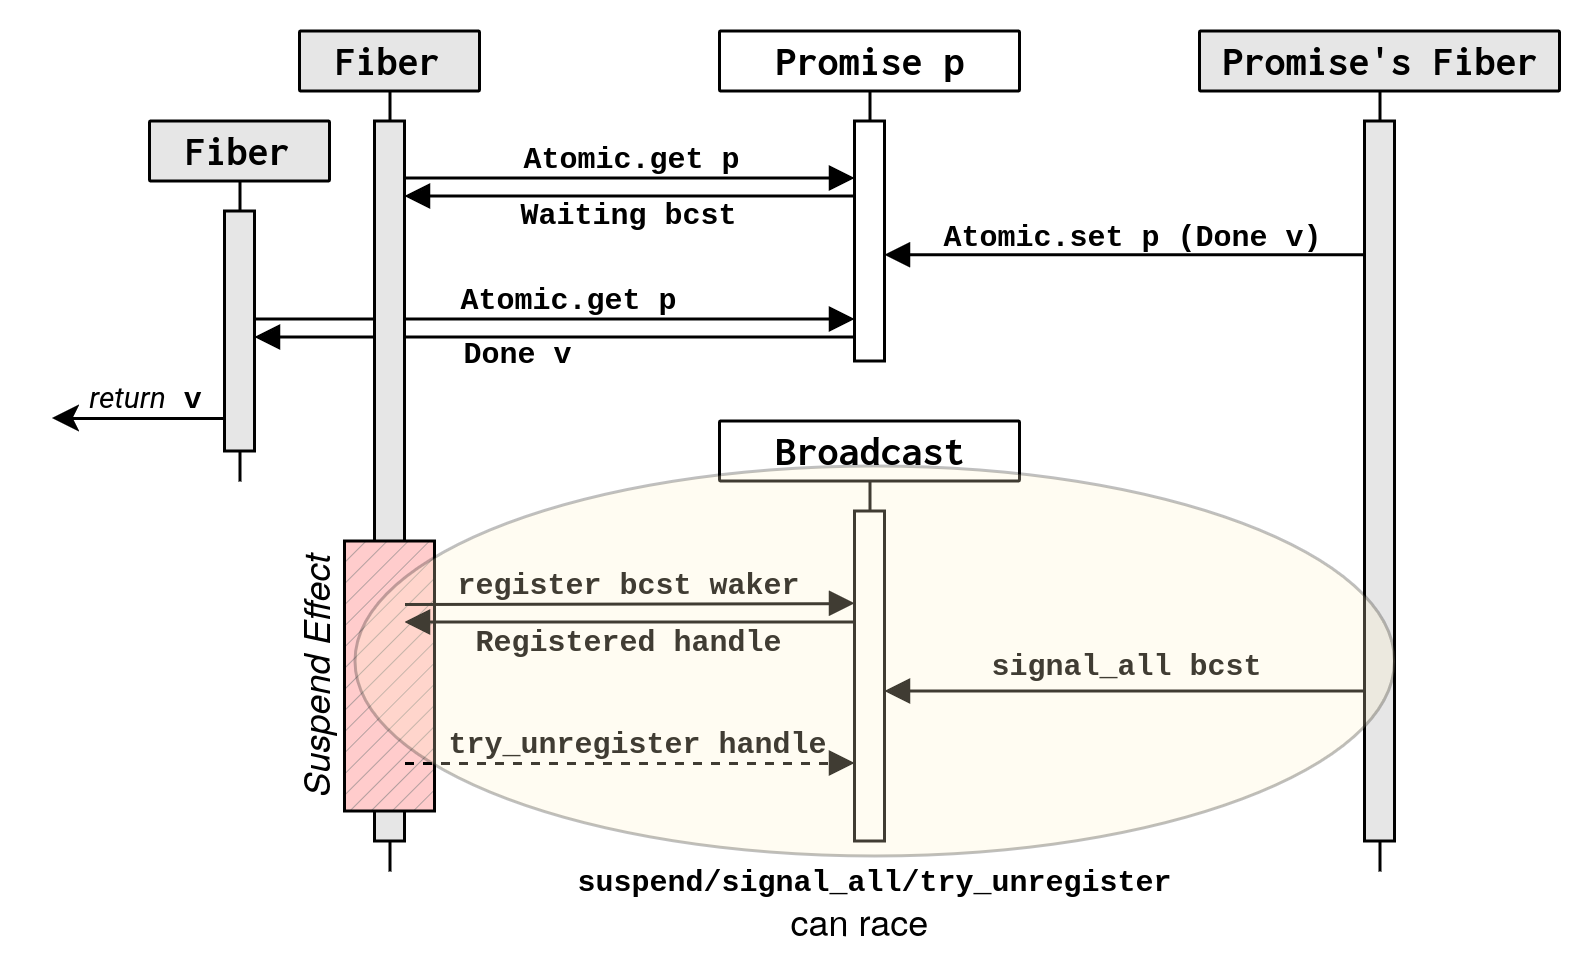
\includegraphics[width=\textwidth]{CQS_Outer_Atomic.png}
  \caption{Usage of Broadcast in the Context of a Promise}
  \label{fig:cqs-usage}
\end{figure}

Note that because it is lock-free and fibers can run on different threads, there can be a race between concurrent register, tryUnregister, and signalAll operations.
Possible interleavings and the necessity of the tryUnregister were explained in section~\ref{sec:sched-impl-await}.

\subsection{Implementation and Logical Interface of Broadcast}
\label{sec:broadcast-impl}

% <!-- Some general information how CQS is implemented and the logical state describing the entire queue. -->

Like the original CQS, broadcast is implemented as a linked list of arrays (called segments) that contain \emph{cells}\footnote{Using segments instead of single cells in the linked list is an optimization to amortize the linear runtime of linked list operations}.
There are two pointers pointing to the beginning and end of the active cell range, the signal pointer and the register pointer, and cells not reachable from either pointer are garbage collected.
There is a set of operations for manipulating the linked list and pointers to implement the higher-level functionality, but they are not part of the public API, so we do not focus on them.
Each cell is a container for one callback and the logical state of the broadcast tracks the logical state of all existing cells.
The possible logical states for a single cell are shown in figure~\ref{fig:cqs-cell-states}, where the arrows are annotated with the operation that causes a state transition.

The logical state of a cell is initialized to \textbf{EMPTY} when it is reached by the register pointer\footnote{As opposed to the original CQS, in broadcast the signal pointer will never overtake the register pointer.}.
When a register and signalAll operation happen concurrently, they race to set the value of the empty cell.
If the signalAll operation wins, it writes a token value into the cell and the logical state becomes \textbf{SIGNALLED}.
The register operation can then read the token and invoke its callback directly.
The logical state is thus \textbf{INVOKED}.
If instead the register operation wins the race, it writes the callback into the cell, so the logical state takes the right path to \textbf{CALLBACK(waiting)}.
Then there can be another race between concurrent tryUnregister and signalAll operations.
Both try to overwrite the callback with a token value, which changes the logical state to \textbf{CALLBACK(invoked)} or \textbf{CALLBACK(unregistered)}, respectively, depending on the winner.

\begin{figure}[ht]
  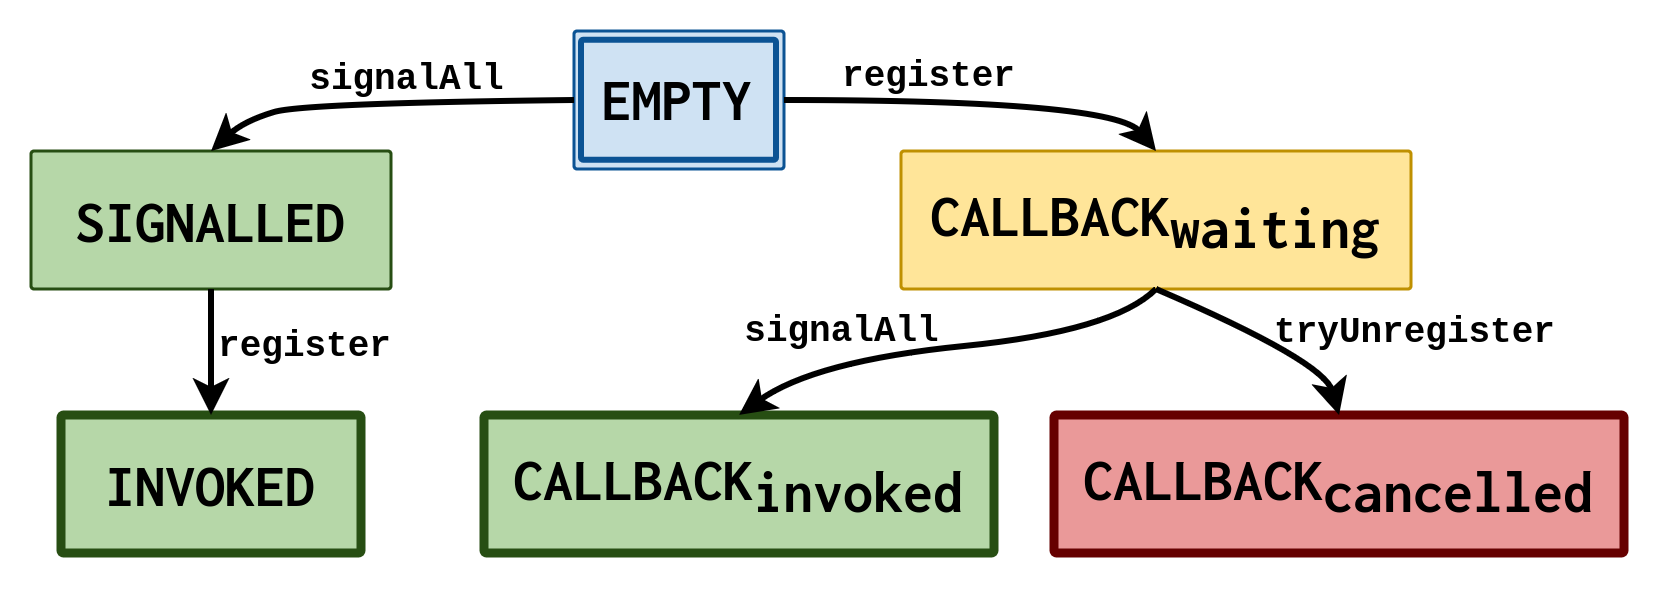
\includegraphics[width=\textwidth]{Cell_States.png}
  \caption{State Transition Diagram for a Single Cell.}
  \label{fig:cqs-cell-states}
\end{figure}

\subsection{Verification of Broadcast}
\label{sec:broadcast-spec}

In the following we describe the specifications we proved for the functions implemented in Eio's \ocamlin{Broadcast} module.
Note that all specifications obey the empty protocol because the code does not perform any effects.
For all three operations, the Eio implementation and specification differs from what is already verified in the original CQS (e.g. due to some reordered instructions or a different control flow).
However, the specifications of the underlying operations for manipulating cell pointers are modular enough to allow us to prove the new specifications for \ocamlin{Broadcast.create}, \ocamlin{Broadcast.register}, and \ocamlin{Broadcast.try_unregister}.

As for \ocamlin{Broadcast.signal_all}, Eio implements this function by atomically increasing the signal pointer by the number \(n\) of registered callbacks and then processing all \(n\) cells between the old and new pointer position.
Because of technical differences in handling these pointers between the original CQS implementation of the paper~\cite{koval2023cqs} and the broadcast implementation of Eio we opted to verify a different implementation of \ocamlin{Broadcast.signal_all}, that increments the signal pointer \(n\) times in a loop.
We argue this does not change the observable behaviors of the function since we ensure that it can only be called once.

\subsubsection{\ocamlin{Broadcast.create}}
\label{sec:broadcast-spec-create}

The only precondition to create a new broadcast is the proposition \(inv\_heap\_inv\).
This is a piece of ghost state defined by the Iris standard library that models invariant locations, which are locations that can always be read.
That means they cannot be explicitly deallocated and can only exist in a garbage-collected setting, like \ocf{}.
The implementation of the linked list uses this internally.

The function returns a broadcast instance \(bcst\), along with the persistent \(\gsIsBcst{}\; bcst\) proposition that shows the value actually is a broadcast.
We also obtain the unique resource \gssignal{}, which is held by the enclosing promise and allows calling the \ocamlin{Broadcast.signal_all} function once.

\[
  \inferrule[Spec-BroadcastCreate]
  {inv\_heap\_inv}
  {\ewp{create\; ()}{\bot}{bcst,\; \gsIsBcst{}\; bcst \ast \gssignal{}}}
\]

\subsubsection{\ocamlin{Broadcast.register}}
\label{sec:broadcast-spec-suspend}

% For a \emph{register} operation the \emph{suspend permit} from the original CQS is not needed anymore since we do the \emph{enqueue registration} internally.
A register operation takes a callback \(cb\) and the associated resource \(\gsIsCb{}\; cb\; R\) which represents the permission to invoke the callback.
We instantiate \(R\) with \gspdone{} so that the callback transports the knowledge that the promise has been fulfilled.
\(\gsIsCb{}\) is not persistent because the callback must be invoked only once.

\begin{align*}
  \gsIsCb{}\; cb\; R                            & \triangleq R \wand \ewp{cb\; ()}{\bot}{\top}                                                           \\
  \emph{isBroadcastRegisterResult}\; r\; cb\; R & \triangleq (\ulcorner r = Called \urcorner)                                                            \\
                                                & \quad \vee (\ulcorner r = Registered\; h \urcorner \ast \emph{isBroadcastRegisterHandle}\; h\; cb\; R) \\
  \emph{isBroadcastRegisterHandle}              & : Val \to Val \to iProp \to iProp
\end{align*}

The \ocamlin{Broadcast.register} function tries to insert a callback into the next cell designated by the register pointer.
If it succeeds the function returns a \ocamlin{Registered handle} value that can be used by \ocamlin{Broadcast.try_unregister}.
But if the cell is already in the \textbf{SIGNALLED} state, the function will immediately invoke the callback and return a \ocamlin{Called} value.

\[
  \inferrule[Spec-BroadcastRegister]
  { \gsIsBcst{}\; bcst \ast \gsIsCb{}\; callback\; R }
  { \ewp{register\; bcst\; callback}{\bot}{r,\; \emph{isBroadcastRegisterResult}\; r\; callback\; R}}
\]

\subsubsection{\ocamlin{Broadcast.try_unregister}}
\label{sec:broadcast-spec-cance}

Given a handle and its \(\textit{isBroadcastRegisterHandle}\; h\; cb\; R\) resource, \ocamlin{Broadcast.try_unregister} will try to cancel the registration of the callback.

If the callback had already been invoked by a call to \ocamlin{Broadcast.signal_all} (i.e. the logical state is \textbf{CALLBACK(invoked)}) the function returns \ocamlin{false} and no resources are returned to the caller.
Otherwise, the permission to invoke the callback \(\gsIsCb{}\; cb\) is returned.

\[
  \inferrule[Spec-BroadcastTryCancel]
  { \emph{isBroadcastRegisterHandle}\; h\; cb\; R }
  { \ewp{try\_unregister\; h}{\bot}{b,\; if\; b\; then\; \gsIsCb{}\; cb\; R\; else\; \top}}
\]

\subsubsection{\ocamlin{Broadcast.signal_all}}
\label{sec:broadcast-spec-signal-all}

To call \ocamlin{Broadcast.signal_all} the unique \(\gssignal{}\) resource is needed, along with a duplicable \(R\), so that it can be used to invoke multiple callbacks.
The function does not return any resources because its only effect is making an unknown number of fibers resume execution, which we cannot easily formalize in Iris.

\[
  \inferrule[Spec-BroadcastSignalAll]
  { \gsIsBcst{}\; bcst \ast \always R \ast \gssignal{}}
  { \ewp{signalAll\; bcst}{\bot}{\top} }
\]

\subsection{Changes from the Original CQS}
\label{sec:broadcast-spec-removed-features}

The original CQS supports multiple additional features like a synchronous mode for suspend and resume, and also a smart cancellation mode.
These features enlarge the state space of CQS and complicate the verification but are not used in Eio so when we ported the verification of CQS to our Eio development we removed support for these features.
This reduced the state space of a cell shown in figure~\ref{fig:cqs-cell-states-original} to a more manageable size when adapting the proofs.

\begin{figure}[ht]
  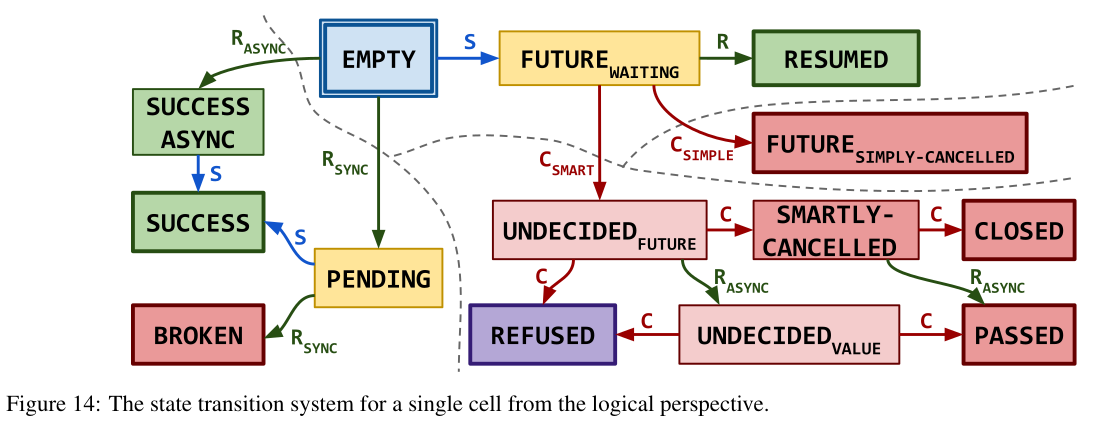
\includegraphics[width=\textwidth]{Cell_States_Original.png}
  \caption{Cell States in the Original CQS from~\cite{koval2023cqs} (page 42).}
  \label{fig:cqs-cell-states-original}
\end{figure}

The part of the verification of the original CQS that we had to customize for Eio was originally 3600 lines of Coq code but -- due to these simplifications -- we could reduce it by approximately 1300 lines of Coq code.
Additionally, there are ~4000 lines of Coq code about lower-level functionality that we did not need to adapt when porting them to our development.

% The number of active cells \(n\) (i.e. the length of the queue) is tracked by the logical resource \(CQSState\; n\).
% In normal usage of CQS, the atomic variable of the outer synchronization construct would encode the length of the queue in its value and keep this resource in an associated invariant.
% Changing the length of the queue is done using \emph{enqueue} and \emph{dequeue registration} logical operations when opening this invariant.

% However, for promises the exact length of the queue is irrelevant because the \emph{signalAll} operation will always set the length to 0.
% So in the adapted proof for Eio's broadcast we keep the \(CQSState\; n\) resource in the invariant of the broadcast itself.
% As a consequence we also move the \emph{enqueue} and \emph{dequeue registration} out of the public logical API because they are now done internally.


\section{Extending the Scheduler with Thread-Local Variables (WIP)}
\label{sec:thread-local-vars}

\begin{itemize}
  \item How thread-local variables can be used.
  \item Explain the GetContext effect in Eio and how we model it in our scheduler.
  \item How we adapt our logical state to include GetContext.
  \item And explain that we need to parameterize the protocol to solve the issue of shared knowledge between the scheduler and fiber.
\end{itemize}

\begin{figure}[ht]
  \begin{alignat*}{2}
    Coop \delta \coloneqq\; &  & \quad Fork\; \#    & \; !\; e\; (e)\; \{\later \ewp{e}{Coop}{\top}\}. ?\; ()\; \{ \top \}          \\
                            &  & Suspend\;    \#    & \; !\; reg\; P\; (reg)\; \{gsIsRegister\; reg\; P\}.?\; y\; (y)\; \{ P\; y \} \\
                            &  & GetContext\;    \# & \; !\; ()\; \{\top\}.?\; ctx\; (ctx)\; \{ isFiberContext\; \delta\; ctx \}
  \end{alignat*}
  \caption{Definition of \proto{} Protocol with \efork{} \& \esuspend{} Effects.}
  \label{fig:coop-protocol-ext}
\end{figure}

% Definition FORK_pre (Coop : pEff) (δ : gname): iEff Σ :=
%   >> (ℓstate : loc) e >> !(Fork' #ℓstate e) {{fiberState δ ℓstate ∗ ▷ (fiberContext δ -∗ EWP e #() <|Coop δ |> {{_, fiberContext δ}}) }};
%   << (_: val) << ?(#())        {{ fiberState δ ℓstate }} @ OS.
%     (* a.d. TODO I think I can delete promiseInv from SUSPEND *)

% Definition SUSPEND (δ : gname) : iEff Σ :=
%   >> (f: val) (P: val → iProp Σ) >> !(Suspend' f) {{
%     (* We call suspender with the waker function and waker receives a value satisfying P. *)
%       ( (∀ (waker: val),
%         (∀ (v: val), P v -∗  (EWP (waker v) <| ⊥ |> {{_, True }}) ) -∗
%         (▷ EWP (f waker) <| ⊥ |> {{_, True  }}) ) 
%     ∗
%       fiberContext δ)%I
%   }};
%   << y           << ?(y)         {{ P y ∗ fiberContext δ }} @ OS.

% Definition GET_CONTEXT (δ: gname ): iEff Σ :=
%   >> (_: val) >> !(GetContext') {{ True }};
%   << (state : loc) << ?(#state) 
%       {{isFiberState δ state}} @ OS.

\section{Evaluation}
\label{sec:evaluation}
We evaluate our model of Eio on a simple example program that uses all features supported by our implementation.
The example program (shown in figure~\ref{fig:eval_code}) may look contrived since it does not do any "useful" computation, but the value of Eio as a library comes from composing computations -- not in what is computed concretely.

The program's \ocamlin{main_fiber} function forks off a new fiber \ocamlin{dispatch} (line~\ref{ln:eval_dispatch}) and communicates with it over a one-element channel represented by the thread-local variable.
The channel is initially empty (first argument to \ocamlin{Scheduler.run} in line~\ref{ln:eval_none}) and \ocamlin{dispatch} polls for data (line~\ref{ln:eval_wait}).
\ocamlin{main_fiber} sends one integer \ocamlin{data} (lines~\ref{ln:eval_receive},\ref{ln:eval_send}) to \ocamlin{dispatch} which will then run two copies of \ocamlin{(work data)} (line~\ref{ln:eval_thread}) in separate threads, and sum their results.
The \ocamlin{work} function simulates time passing using the \ocamlin{yield} function (line~\ref{ln:eval_work}) and returns its first argument.
Yield performs a \esuspend{} effect but calls the \ocamlin{waker} function immediately, which has the effect of placing the current fiber at the back of the scheduler's run queue to give other fibers a chance to run.

The example program therefore uses the basic functions for forking and awaiting the completion of fibers, multiple schedulers running in different threads, as well as thread-local variables to communicate between fibers within one thread.

\begin{figure}[ht]
    \begin{minted}[escapeinside=@@]{ocaml}
let yield () = @\label{ln:eval_yield}@ 
  perform (Suspend (fun waker -> waker ()))

let work x () = 
  yield (); @\label{ln:eval_work}@
  x

let rec wait_for_data (tlv : tlv ref) =
  match !tlv with
  | None -> yield (); wait_for_data tlv
  | Some data -> tlv := None; data @\label{ln:eval_receive}@

let dispatch () =
  let tlv = perform (GetContext ()) in
  let data = wait_for_data tlv in @\label{ln:eval_wait}@
  let p1 = Fiber.fork_promise (fun () -> Domain_manager.new_scheduler (work data)) in @\label{ln:eval_thread}@
  let p2 = Fiber.fork_promise (fun () -> Domain_manager.new_scheduler (work data)) in
  let r1 = Promise.await p1 in
  let r2 = Promise.await p2 in
  r1 + r2

let main_fiber data () =
  let p = Fiber.fork_promise dispatch in @\label{ln:eval_dispatch}@
  let tlv = perform (GetContext ()) in
  tlv := Some data; @\label{ln:eval_send}@
  Promise.await p

let main () = 
  Scheduler.run None (main_fiber 21) @\label{ln:eval_none}@
\end{minted}
    \caption{Example program to use all implemented features.}
    \label{fig:eval_code}
\end{figure}

We first give the final specifications of the most important components of our model library in figure~\ref{fig:eval-total}.
The specifications contain both extensions we discussed in sections~\ref{sec:domain-manager} and~\ref{sec:thread-local-vars}.

\begin{figure}[ht]
    \begin{align*}
        \gsReadyF{}~l~\Omega~\gamma~q~k & \triangleq \begin{aligned}[t]
                                                         & \gsFiberResources{l}{\Omega} \wand                                                                                                           \\
                                                         & \later isQueueReader~q~(\gsReadyF{}~l~\Omega~\gamma~q) \wand                                                                                  \\
                                                         & \quad \ewp{k~()}{\bot}{\_.\; \gsFiberResources{l}{\Omega} \ast \later isQueueReader~q~(\gsReadyF{}~l~\Omega~\gamma~q) \ast \gspdone{\gamma} }
                                                    \end{aligned} \\
        \gsIsWaker{}~wkr~W             & \triangleq \forall v.   \;  W\; v \wand{} \ewp{wkr\ \ v}{\bot}{\top}                                                                                                \\
        \gsIsRegF{}~reg~W~S             & \triangleq \forall wkr. \; \gsIsWaker{}\; wkr\; W \wand{} \ewp{reg\ \ wkr}{\bot}{\always S}                                                                         \\
        \protoF{}~l~\Omega              & \triangleq \begin{aligned}[t]
                                                        Fork\;       & \#\; \begin{aligned}[t]
                                     & !\; e\; ((l, e))\; \begin{aligned}[t]
                                           & \big\{ \gsFiberResources{l}{\Omega} \ast                                                                              \\
                                           & \later\; (\gsFiberResources{l}{\Omega} \wand{} \ewp{e\ \ ()}{\protoF{}~l~\Omega}{\gsFiberResources{l}{\Omega}}) \big\}
                                      \end{aligned} . \\
                                     & ?\; ()\; \{ \gsFiberResources{l}{\Omega} \}
                                \end{aligned}                                             \\
                                                        Suspend\;    & \#\; \begin{aligned}[t]
                                     & !\; reg\; W\; S\; (reg)\; \{\gsFiberResources{l}{\Omega} \ast \gsIsRegF{}\; reg\; W\; S\}. \\
                                     & ?\; v\; (v)\; \{ \gsFiberResources{l}{\Omega} \ast W~v \ast S \}
                                \end{aligned} \\
                                                        GetContext\; & \#\; !\; ()\; \{\top\}.\; ?\; (l)\; \{ \top \}
                                                    \end{aligned}
    \end{align*}
    \begin{mathpar}
        \inferrule[Spec-Run]
        { \Omega~init \;\ast \\\\ \forall l_{tlv}.\; \gsFiberResources{l_{tlv}}{\Omega} \wand \ewp{main\ \ ()}{\protoF{}~l_{tlv}~\Omega}{v.\; \always \Phi~v \ast \gsFiberResources{l_{tlv}}{\Omega}} }
        { \ewp{run\ \ init\ \ main}{\bot}{v.\; \always \Phi~v \ast \gsFiberResources{l_{tlv}}{\Omega}} }
        %
        \and
        %
        \inferrule[Spec-ForkPromise]
        { \gsPInv{} \ast \gsFiberResources{l_{tlv}}{\Omega} \;\ast \\\\ \gsFiberResources{l_{tlv}}{\Omega} \wand \ewp{f\ \ ()}{\protoF{}~l_{tlv}~\Omega}{v.\; \always \Phi~v \ast \gsFiberResources{l_{tlv}}{\Omega}} }
        { \ewp{fork\_promise\ \ f}{\protoF{}~l_{tlv}~\Omega}{p.\; \gsIsPr{}~p~\Phi \ast \gsFiberResources{l_{tlv}}{\Omega}} }
        %
        \and
        %
        \inferrule[Spec-Await]
        { \gsPInv{} \ast \gsFiberResources{l_{tlv}}{\Omega} \ast \gsIsPr{}~p~\Phi }
        { \ewp{await\ \ p}{\protoF{}~l_{tlv}~\Omega}{p.\; \gsIsPr{}~p~\Phi \ast \gsFiberResources{l_{tlv}}{\Omega}} }
        %
        \and
        %
        \inferrule[Spec-NewScheduler]
        { \Omega'~init \;\ast \\\\ \forall l'_{tlv}.\; \gsFiberResources{l'_{tlv}}{\Omega} \wand \ewp{main\ \ ()}{\protoF{}~l'_{tlv}~\Omega'}{v.\; \always \Phi~v \ast \gsFiberResources{l'_{tlv}}{\Omega'}} }
        { \ewp{new\_scheduler\ \ init\ \ main}{\protoF{}~l~\Omega}{v.\; \always \Phi~v \ast \gsFiberResources{l}{\Omega}} }
    \end{mathpar}

    \caption{Specification of the public interface of the Eio library model.}
    \label{fig:eval-total}
\end{figure}

Using these specifications we proved the safety of the example program and its functional correctness by establishing specifications for each function as shown in figure~\ref{fig:eval-spec}.
We can see that there is some amount of boilerplate (colored in {\color{blue} blue}).
Each function that yields execution to another fiber by performing an effect -- either directly or indirectly through another function call -- needs \({\color{blue}\gsFiberResources{l_{tlv}}{\Omega}}\), which signifies the ownership over the thread-local variable.
Additionally, any fiber that wants to fork off another fiber using \ocamlin{Fiber.fork_promise} needs the persistent \({\color{blue}\gsPInv{}}\) resource to interact with the global collection of promises.
The predicate \(\Omega_{chan}~\gamma\) as part of \(\gsFiberResources{l_{tlv}}{(\Omega_{chan}~\gamma)}\) restricts the thread-local variable \(l_{tlv}\) to be a channel for a single message \(n\).

\begin{figure}[ht]
    \begin{align*}
        \Omega_{chan}~\gamma~v & \triangleq \begin{aligned}[t]
                                                       & \ulcorner v = None \urcorner                                                    \\[-5pt]
                                                \vee\; & \exists n.\; \ulcorner v = Some~n \urcorner \ast \ownGhost{\gamma}{\aginj{}(n)}
                                            \end{aligned} \\
    \end{align*}
    \begin{mathpar}
        \inferrule[Spec-Work]
        { {\color{blue}\gsFiberResources{l_{tlv}}{\Omega}} }
        { \ewp{work\ \ n\ \ ()}{\protoF{}~l_{tlv}~\Omega}{v.\; \ulcorner v = n \urcorner \ast {\color{blue}\gsFiberResources{l_{tlv}}{\Omega}}} }
        %
        \and
        %
        \inferrule[Spec-WaitForData]
        { {\color{blue}\gsFiberResources{l_{tlv}}{(\Omega_{chan}~\gamma)}} }
        { \ewp{wait\_for\_data\ \ l}{\protoF{}}{v.\; \exists n.\; \ulcorner v = n \urcorner \ast \ownGhost{\gamma}{\aginj{}(n)} \ast {\color{blue}\gsFiberResources{l_{tlv}}{(\Omega_{chan}~\gamma)}}} }
        %
        \and
        %
        \inferrule[Spec-Dispatch]
        { {\color{blue}\gsPInv{}} \ast {\color{blue}\gsFiberResources{l_{tlv}}{(\Omega_{chan}~\gamma)}} }
        { \ewp{dispatch\ \ ()}{\protoF{}}{v.\; \exists n.\; \ulcorner v' = n + n \urcorner \ast \ownGhost{\gamma}{\aginj{}(n)} \ast {\color{blue}\gsFiberResources{l_{tlv}}{(\Omega_{chan}~\gamma)}}} }
        %
        \and
        %
        \inferrule[Spec-MainFiber]
        { {\color{blue}\gsPInv{}} \ast {\color{blue}\gsFiberResources{l_{tlv}}{(\Omega_{chan}~\gamma)}} \ast \ownGhost{\gamma}{\aginj{}(n)} }
        { \ewp{main\_fiber\  n\  ()}{\protoF{}}{v.\; \ulcorner v = n + n \urcorner \ast {\color{blue}\gsFiberResources{l_{tlv}}{(\Omega_{chan}~\gamma)}}} }
        %
        \and
        % 
        \inferrule[Spec-Main]
        { }
        { \ewp{main\ \ ()}{\bot}{v.\; \ulcorner v = 42 \urcorner} }
    \end{mathpar}
    \caption{Specification of the example program.}
    \label{fig:eval-spec}
\end{figure}

While we proved the safety of this program (and of the core abstractions of the Eio library), the complete Eio library has more features that are still unexplored.
This includes cancellation of fibers, resource management using switches and several operating system primitives like timers, so we cannot make any statements about programs using these features.
Nevertheless, our model is an important step in the direction of proving the safety of Eio and programs that use it.
Iris along with its features like ghost state and shareable invariants to reason about multithreaded and stateful code were key in this development.


\section{Conclusion}
\label{sec:conclusion}

\subsection{Related Work}
\paragraph*{Concurrency With Effects}
There are other approaches to implementing cooperative concurrency with effects even within \ocf{}.
One example is the Picos framework~\cite{Picos}, an interoperability framework that defines a small set of data types and effects that can be reused by other cooperative concurrency libraries (such as Eio)
in order to speak a common protocol and be mutually interoperable.
Picos defines \emph{computations} and \emph{fibers}, which are mostly equivalent, respectively, to Eio's promises and fibers.
The main difference is the \emph{trigger} concept, which in Eio's terms can be thought of as a mutable reference to an optional \ocamlin{waker} function.
% The workflow to await a result in Eio is to, first define a \ocamlin{register} function and perform a \esuspend{} effect with it. 
% The scheduler will call the \ocamlin{register}
The workflow to await a future result (i.e. a Picos computation) resembles Landin's Knot in that it consists of first attaching an empty trigger to the computation and then assigning a \ocamlin{waker} function later.
This is done by performing an \emph{Await} effect after attaching the trigger so that the effect handler (implemented by a library such as Eio) then creates a \ocamlin{waker} function and assigns it to the trigger.
When the computation finishes it will signal the trigger, which calls the \ocamlin{waker} function and consequently places the original fiber in the scheduler's run queue.

While the \emph{Await} effect carrying a trigger is technically first-order -- as opposed to Eio's higher-order \esuspend{} effect carrying a \ocamlin{register} function --
a trigger still contains higher-order state.
So it is unclear to us whether a specification for the Picos primitives would be any simpler to prove or easier to use than the specification for Eio primitives we have presented so far.

\paragraph*{Session Types as Effect Specifications}
Protocols in \hazel{} take some inspiration from session types but with the restriction that a protocol is always an infinite repetition of a single step, whereas session types usually allow defining a sequence of different steps.
Current work by Tang~\cite{tangeff} explores the connection between session types and effect protocols further and defines a lambda calculus \(\lambda^{\mbox{{\footnotesize \Letter}}}_{\mathrm{eff}}\) that uses a standard session type formalization
for its effect system.
This allows a programmer to define multistep protocols and even bidirectional effects where the handler and client swap roles.
However, for our purposes \hazel{} is completely sufficient since multistep protocols can be simulated by \hazel{}'s protocols and bidirectional effects are not possible in \ocf{} to begin with.

% \paragraph*{}
% Current work by van Rooij~\cite{?} extends the type and effects system Tes of de Vilhena~\cite{de2022proof} to track in the type system whether a continuation is one- or multi-shot.

% \paragraph*{Other Verifications of Eio Primitives}
% \todo{There seems to be something called zebre that is referenced by Eio and implements at least the Lf\_queue of Eio \url{https://github.com/clef-men/zebre/} but otherwise appears to model a different kind of scheduler.}

\subsection{Future Work}
The work we presented so far suffices to prove the safety of programs that use a small subset of the full functionality provided by Eio.
To improve the usefulness of our model and be applicable to more programs it would be desirable to incorporate more features into our model of Eio in future work, such as switches and support for cancelling fibers.
While switches are mainly used for a hierarchical organization of fibers and to efficiently clean up fiber resources, cancellation poses some interesting safety questions because there are situations that must be avoided, such as being able to cancel a fiber twice.

Instead of growing the model of Eio it would also be interesting to extend the existing specifications.
Mainly, we would be interested in proving that a scheduler will never "forget fibers".
Since weakest preconditions in Iris do not prove termination our specifications have the unfortunate drawback of being fulfilled by functions that diverge.
Because a scheduler explicitly handles fiber continuations it would be possible to accidentally drop a continuation which has the effect of making the fiber diverge, as well as any other fiber that awaits its result.

While we cannot solve the whole termination problem (since deadlocks are possible), intuitively we should be able to track the state of each fiber to ensure that when a fiber is captured in a continuation,
the continuation is used linearly, which means that it is explicitly invoked or discarded at some point.
This also extends to data structures that contain continuations like the scheduler's run queue and a broadcast, as they must never drop the contained continuations.
To track the linear usage of continuations it could be helpful to draw inspiration from Iron~\cite{bizjak2019iron}, a separation logic built on Iris to enable reasoning about linear resources.

% Finally, to make the statement "the program can diverge but not due to mishandled continuations" formal, it might be possible to use Transfinite Iris~\cite{spies2021transfinite} and prove a \emph{termination-preserving refinement} 
% of the scheduler to a simpler scheduler where the linear handling of fiber continuations is more easily provable.
% However, it is non-obvious how such a simpler scheduler would look like since termination of the whole program 

\subsection{Results}

In this thesis we have proven specifications for a subset of the Eio library, including a common denominator scheduler that controls fibers which can await the completion of promises in a multithreaded setting.
We have also defined and verified general and reusable protocols for the main three effects of Eio: \efork{}, \esuspend{}, and \egetctx{}.
We showed that the function specifications and the effect protocols are enough to verify the safety (including effect safety) of an example program that uses all of our modelled features.
Additionally, we have verified specifications for two nontrivial data structures used by Eio.
For the broadcast data structure we adapted the existing proof of CQS by Koval et al.~\cite{koval2023cqs}
and for the scheduler's run queue we proved a -- to our knowledge novel -- specification for a multi-producer single-consumer queue with a temporarily suspendable invariant.
Finally, we have extended the original \hh{} language with multithreading primitives and amended the adequacy result which shows that we can use this language to reason about programs that use both multithreading and effect handlers.


\section*{Appendix}
\label{sec:appendix}


\subsection*{A. Translation Table}
\label{sec:apdx-translation}

\begin{table}[ht]
	\begin{tabular}{l|l|l}
		Eio                          & Thesis                       & Mechanization          \\
		\hline
		\ocamlin{enqueue}            & \ocamlin{waker} function     & \ocamlin{waker}        \\
		\ocamlin{f}                  & \ocamlin{register} function  & \ocamlin{register}     \\
		\ocamlin{Fiber.fork_promise} & \ocamlin{Fiber.fork_promise} & \ocamlin{fork_promise} \\
		\ocamlin{Promise.await}      & \ocamlin{Promise.await}      & \ocamlin{await}        \\
		\ocamlin{Sched.run}          & \ocamlin{Scheduler.run}      & \ocamlin{run}          \\
	\end{tabular}
\end{table}

\subsection*{B. Towards A Multi-Threaded Scheduler}
\label{sec:apdx-mt}

OCaml 5 added not only effect handlers but also the ability to use multiple threads of execution, which are called \textit{domains} (in the following we use the terms interchangeably).
Each domain in OCaml 5 corresponds to one system-level thread and the usual rules of multi-threaded execution apply, i.e. domains are preemtively scheduled and can share memory.
Eio defines an operation to make use of multi-threading by forking off a new thread and running a separate scheduler in it.
So while each Eio scheduler is only responsible for fibers in a single thread, fibers can await and communicate with fibers running in other threads.

In order for a fiber to be able to await fibers in another thread, the \ocamlin{wakers_queue} [note it will be in the Simple Scheduler section] from above is actually a thread-safe queue based on something called CQS, which we will discuss in detail in a later section.

Heaplang supports reasoning about multi-threaded programs by implementing fork and join operations for threads and defining atomic steps in the operational semantics, which enables the use of Iris \textit{invariants}.
In contrast, Hazel did not define any multi-threaded operational semantics but it contained most of the building blocks for using invariants.
In the following we explain how we added a multi-threaded operational semantics and enabled the use of invariants.

% \ocamlin{}`
% Aside: Memory Model in OCaml 5
% In the OCaml 5 memory model, \textit{atomic variables} are needed in order to access shared memory without introducing data races.
% Instead of modelling atomic variables in Hazel, we continue to use normal references because the multi-threaded operational semantics by definition defines all memory operations to be sequentially consistent. This seems to be the standard approach and is done the same way in Heaplang.
% \ocamlin{}`

\subsubsection*{Adding Invariants to Hazel}

Invariants in Iris are used to share resources between threads.
They encapsulate a resource to be shared and can be opened for a single atomic step of execution.
During this step the resource can be taken out of the invariant and used in the proof but at the end of the step the invariant must be restored.

Hazel did already have the basic elements necessary to support using invariants.
It defined a ghost cell to hold invariants and proved an invariant access lemma which allows opening an invariant if the current expression is atomic.
In order to use invariant we only had to provide proofs for which evaluation steps are atomic.
We provided proofs for all primitive evaluation steps.
The proofs are the same for all steps so we just explain the one for \ocamlin{Load}.

\begin{minted}{coq}
Lemma ectx_language_atomic a e :
head_atomic a e → sub_exprs_are_values e → Atomic a e.

Instance load_atomic v : Atomic StronglyAtomic (Load (Val v)).
Instance store_atomic v1 v2 : Atomic StronglyAtomic (Store (Val v1) (Val v2)).
...
\end{minted}

An expression is atomic if it takes one step to a value, and if all subexpressions are already values.
The first condition follows by definition of the step relation and the second follows by case analysis of the expression.

Since performing an effect starts a chain of evaluation steps to capture the current continuation, it is not atomic.
For the same reason an effect handler and invoking a continuation are not atomic except in degenerate cases.
Therefore, invariants and effects do not interact in any interesting way.
\todo{How we add support for the iInv tactic to use invariants more easily.}

\subsubsection*{Adding Multi-Threading to Hazel}

To allow reasoning in Hazel about multi-threaded programs we need a multi-threaded operational semantics as well as specifications for the new primitive operations \efork{}, \ocamlin{Cmpxcgh} and \ocamlin{FAA}.

The language interface of Iris provides a multi-threaded operational semantics that is based on a thread-pool.
The thread-pool is a list of expressions that represents threads running in parallel.
At each step, one expressions is picked out of the pool at random and executed for one thread-local step.
Each thread-local step additionally returns a list of forked-off threads, which are then added to the pool.
This is only relevant for the \efork{} operation as all other operations naturally don't fork off threads.

% (e, \sigma) ->_t (e', \sigma', es')
% ------------------------------------------------------------
% (es_1 ++ e ++ es_2, \sigma) ->_mt (es_1 ++ e' ++ es_2 + es', \sigma')

Heaplang implements multi-threading like this and for Hazel we do the same thing.
We adapt Hazel's thread-local operational semantics to include \efork{}, \ocamlin{Cmpxchg} and \ocamlin{FAA} operations and to track forked-off threads and get a multi-threaded operational semantics "for free" from Iris' language interface.

Additionally, we need to prove specifications for these three operations.
\ocamlin{Cmpxchg} and \ocamlin{FAA} are standard so we will not discuss them here.
The only interesting design decision in the case of Hazel is how effects and \efork{} interact.
This decision is guided by the fact that in OCaml 5 effects never cross thread-boundaries.
An unhandled effect just terminates the current thread.
As such we must impose the empty protocol on the argument of \efork{}.

% EWP e <| \bot |> { \top }
% -------------------------------------
% EWP (Fork e) <| \Phi |> { x, x = () }

Using these primitive operations we can then build the standard \ocamlin{CAS}, \ocamlin{Spawn}, and \ocamlin{Join} operations on top and prove their specifications.
For \ocamlin{Spawn} \& \ocamlin{Join} we already need invariants as the point-to assertion for the done flag must be shared between the two threads.

% Lemma spawn_spec (Q : val → iProp Σ) (f : val) :
% EWP (f #()) <| \bot |> {{ Q }} -∗ EWP (spawn f) {{ v, ∃ (l: loc), ⌜ v = #l ⌝ ∗ join_handle l Q }}.

% Lemma join_spec (Q : val → iProp Σ) l :
% join_handle l Q -∗ EWP join #l {{ v, Q v }}.

% Definition spawn_inv (γ : gname) (l : loc) (Q : val → iProp Σ) : iProp Σ :=
% ∃ lv, l ↦ lv ∗ (⌜lv = NONEV⌝ ∨
% ∃ w, ⌜lv = SOMEV w⌝ ∗ (Q w ∨ own γ (Excl ()))).

% Definition join_handle (l : loc) (Q : val → iProp Σ) : iProp Σ :=
% ∃ γ, own γ (Excl ()) ∗ inv N (spawn_inv γ l Q).

Note that for \ocamlin{Spawn} we must also impose the empty protocol on \ocamlin{f} as this expression will be forked-off.

This allows us to implement standard multi-threaded programs which also use effect handlers.
For example, we can prove the specification of the function below that is based on an analogous function in Eio which forks a thread and runs a new scheduler inside it.
Note that same as in Eio the function blocks until the thread has finished executing, so it should be called in separate fiber.

% Definition spawn_scheduler : val :=
% (λ: "f",
% let: "new_scheduler" := (λ: <>, run "f") in
% let: "c" := spawn "new_scheduler" in
% join "c")%V.

% Lemma spawn_scheduler_spec (Q : val -> iProp Σ) (f: val) :
% promiseInv -∗ EWP (f #()) <| Coop |> {{ _, True }} -∗
% EWP (spawn_scheduler f) {{ _, True }}.

The scheduler \ocamlin{run} and therefore also the \ocamlin{spawn_scheduler} function don't have interesting return values, so this part of the specification is uninteresting.
What is more interesting is that they encapsulate the possible effects the given function \ocamlin{f} performs.

\subsection*{C. A Note on Cancellation}
\label{sec:apdx-cancellation}

\begin{itemize}
	\item That we tried to model cancellation but the feature is too permissive to give it a specification.
	\item There is still an interesting question of safety (fibers cannot be added to a cancelled Switch).
	\item But including switches \& cancellation in our model would entail too much work so we leave it for future work.
\end{itemize}


\printbibliography

\end{document}